\documentclass[11pt, twoside]{article}	% Always compile at least twice.
\listfiles
\usepackage[lmargin=1in,rmargin=1in,tmargin=1in,bmargin=1in]{geometry}

% Cover Information
\def\univname{Midwestern State University}
\def\coursenum{CMPS 3013}
\def\coursetitle{Algorithms}
\def\coursesubtitle{Course Notes}
\def\professor{Griffin}
% \def\student{Note Taker}
\def\semesteryear{Spring 2021}
\def\imagename{images/msutexas3}		    % Replace with University Seal
\def\scalesize{0.90}					% Scale Logo Size 

% Style Package (Load After Cover Information)
\usepackage{course}	% Change to match style file

% Generate the glossary
% https://texblog.org/2014/01/15/glossary-and-list-of-acronyms-with-latex/
% \newglossaryentry{⟨label⟩}{name={⟨key⟩}, description={⟨value⟩}}

\setglossarystyle{list}
\setglossarystyle{altlist}
\setglossarystyle{listgroup}
\setglossarystyle{listhypergroup}
% list. Writes the defined term in boldface font
% altlist. Inserts newline after the term and indents the description.
% listgroup. Group the terms based on the first letter.
% listhypergroup. Adds hyperlinks at the top of the index.

\makeglossaries

% -------------------
% Content
% -------------------
\begin{document}
\fontfamily{phv}\selectfont
\color{reg}
 
% Cover Page
\coverpage

% Last Updated
\updated{\today}

% Table of Contents
\thispagestyle{empty}
\tableofcontents
\newpage
\pagestyle{fancy}
\setcounter{section}{0}
\setcounter{page}{1}

% Sections

% \newpage
\mysection{Introduction \label{sec:crypthints}}

 This course is called "Advanced Structures and Algorithms" and its essence is learning how to create complex structures along with the algorithms that provide efficient ways to store and retrieve data from within those structures. The Efficiency of an advanced structure is something you will learn to measure by evaluating the \ccb{run times} (aka costs) of each algorithm we explore, and how the data structure used for storing the data may impact overall efficiency.\\
 
 In my opinion, this course is your first "real" programming course. Some students feel that data structures (1063) was a tough course, and I don't disagree, however this course will require you to use all the skills you gained ... and then some. If you struggle with arrays, pointers, or linked lists you may want to come see me, or review the following materials:
 
 \begin{enumerate}
    \item \href{https://cs.msutexas.edu/~griffin/materials/Arrays.pdf}{Arrays}
    \item \href{https://cs.msutexas.edu/~griffin/materials/PointersAndMemory.pdf}{Pointers and Memory}
    \item \href{https://cs.msutexas.edu/~griffin/materials/LinkedListBasics.pdf}{Linked List Basics}
\end{enumerate}

\mysubsection{Array vs List}

I just eluded to the fact that your previous course had a goal of getting you comfortable with certain concepts. One of those concepts was: "Do I use an array to store my data? Or do I used a linked list?"  In computer science we use the terms: \ccb{array based structure} and \ccb{list based structure} for our two choices on how to store data in memory. However, to create list based structures you need to "link" memory locations, and so you were introduced to \ccb{pointers} which allowed you to create \ccb{linked lists}. Both arrays and linked lists have pros and cons associated with them, and understanding the pros and cons of each structure will help you understand why certain algorithms work better when implemented using one or the other. There is not a single best choice, an array can do anything a linked list can, and vice versa. But in certain situations, one will be better than the other. This course will help you know when to choose one over the other. Below is a summary of both: \\

\ccb{Array:}\\
\vspace{-.5cm}
\begin{enumerate}
    \item Direct access (random access) using subscript.
    \item Growing and shrinking is costly.
    \item Bad for lots of insertions and deletions (because of empty slots and need for shifting).
    \item Good for searching (if items are ordered).
\end{enumerate}

\ccb{Linked Lists: }\\
\vspace{-.5cm}
\begin{enumerate}
    \item Access requires traversal using a pointer.
    \item Grows and shrinks easily.
    \item Good for lots of insertions and deletions (because of previous point).
    \item Bad for searching (linear only).
\end{enumerate}

\begin{center}
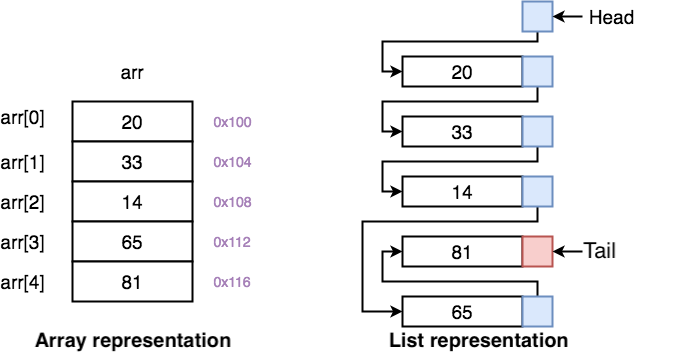
\includegraphics[scale=.35]{images/array-vs-linked-list.png}
\end{center}

\begin{table}[ht]
\footnotesize
    \centering
    \begin{tabular}{|p{3cm}|p{5.5cm}|p{6cm}|}
        \hline
        \textbf{Comparison} & \textbf{Array} & \textbf{Linked List} \\
        \hline
        Generic & Contiguous memory locations of fixed size.& Dynamically allocated memory locations linked by pointers. \\
        \hline
        Size & Fixed at allocation. & Grows and shrinks easily. \\
        \hline
        Order of the elements &	Stored consecutively & Stored randomly\\
        \hline
        Accessing  & Direct access using subscript. & Sequentially accessed from head or other pointer. \\
        \hline
        Insertion and deletion & Slow if shifting is required. & Easier, fast and efficient.\\
        \hline
        Searching &	Binary search (if ordered values) and linear search. & Linear search only.\\
        \hline
        Memory required & Size of data stored.	& Size of data stored + pointer.\\
        \hline
    \end{tabular}
    \caption{Array VS Linked List\supcite{arrayvlinked}}
    \label{table:listvarray}
\end{table}

\mysubsection{Stacks and Queues}

Something else you should have taken away from your previous CS course is the concepts of two simple data structures: 1) \ccb{Stacks} and 2) \ccb{Queues}. Not only the concept of how they work (LIFO v FIFO), but also how to implement either of them using an array or a list.

 \begin{enumerate}
    \item \href{https://cs.msutexas.edu/~griffin/materials/StacksAndQueues.pdf}{Stacks and Queues Helper Material}
\end{enumerate}

There are many other things you should have taken away from your data structures course, but to continue in this class with some comfort, you really should comfortably grasp the following. Each of the items is a link to a gist with example code. 

 \begin{enumerate}
    \item \href{https://gist.github.com/rugbyprof/1ebeeb6a5942050b8e326762f114cddd}{Array Based Stack}
    \item \href{https://gist.github.com/rugbyprof/84fd677220eeae40bdc7be07600f6f58}{List Based Stack}
    \item \href{https://gist.github.com/rugbyprof/3960ce651ae5397f525b1d83a69fa899}{Array Based Queue}
    \item \href{https://gist.github.com/rugbyprof/cb9bb1627d234e0987369028da524197}{List Based Queue}
\end{enumerate}

If you can comfortably write all of those combinations basically from scratch, you are in a good position to continue. If not, practice!! 

\mysubsection{Algorithm vs Data Structure}

We have laid the groundwork and are ready to discuss what \textit{advanced structures \& algorithms} really are. They are (to put it another way) \textit{advanced \underline{data} structures \textbf{and the} algorithms \underline{used to} \underline{manipulate them}}. They are two separate concepts, but in this context they are highly related. Lets look at each term separately.\\

\textbf{Data Structure:} In computer science, a \textit{data structure} is a data organization, management, and storage format that enables efficient access and modification. More precisely, a data structure is a collection of data values, the relationships among them, and the functions or operations that can be applied to the data\supcite{wiki:ds}.\\

\textbf{Algorithm:} In mathematics and computer science, an \textit{algorithm}  is a finite sequence of well-defined, computer-implementable instructions, typically to solve a class of problems or to perform a computation. Algorithms are always unambiguous and are used as specifications for performing calculations, data processing, automated reasoning, and other tasks\supcite{wiki:alg}.\\ 

Both of these fundamental blocks are needed to solve problems in computer science, and are also why our field is so tightly coupled with mathematics. A good data structure allows for the efficient storage and retrieval of data. But to make this happen we (typically) need to follow a sequence of well-defined instructions to guarantee \textit{unambiguous} behavior by our data structure \footnote{Describe what "ambiguous" behavior of an algorithm or data structure might be}. What exactly does that mean? Let's use an example to clarify.\\

\mysubsection{Stack vs Queue Example}

Let me explain how the two relate by providing an example using concepts you have already been introduced to. When implementing a data structure, you have two choices for your \ccb{storage format}: 1) Array Based or 2) a List Based structure\footnote{Or some hybrid of the two. But in general, those are the choices}. In other words I can use an \ccb{array} or I can use a \ccb{linked list} to implement my stack or queue. But what exactly makes an array or a linked list a \ccb{stack} or a \ccb{queue}? They both have push operations. They both have pop operations\footnote{Some books use 'enqueue' and 'dequeue' as operations for a queue, but they still add and remove items.}. The difference is in the algorithm that you employ to add or retrieve that data. A stack uses \ccb{LIFO} (Last In First Out) while a queue uses \ccb{FIFO} (First In First Out). A small change in the algorithm you use to implement the data structure changes the entire behavior of that data structure regardless of the \textit{storage format} that you chose. The algorithm that we use to add or remove items from each structure will guarantee, unambiguously, that the data structure will behave in a correct manner. \\

Let's look at the difference in algorithms between a stack and a queue. This example will use an array as its storage container. See the implementation of \ccb{Push} and \ccb{Pop} below: \\

\begin{table}[H]
\begin{tabular}{|M{0.1\textwidth}|m{0.45\textwidth}|m{0.45\textwidth}|}
    \hline
    \textbf{Op} & \textbf{Stack} & \textbf{Queue} \\
    \hline
    
    \textbf{Push} 
    &
    \begin{minipage}[t]{0.5\textwidth}
    \begin{minted}[]{c++}
    //
    bool Push(int x){
        if(!full()){
            ++top;
            array[top] = x;
            return true;
        }
        return false;
    }
    \end{minted}
    \end{minipage}
    &
    \begin{minipage}[t]{0.5\textwidth}
    \begin{minted}[bgcolor=clear]{c++}
    bool Push(int x){
        if(!full()){
            array[rear] = x;
            rear = (rear + 1) % array_size;
            return true;
        }
        return false;
    }
    \end{minted}
    \end{minipage}\\
    \hline
    \textbf{Pop} 
    &
    \begin{minipage}[t]{0.5\textwidth}
    \begin{minted}[]{c++}
    //
    int Pop(){
        if(!empty()){
            int retval = array[top];
            --top;
            return retval;
        }
        return INT_MIN;
    }
    \end{minted}
    \end{minipage}
    &\begin{minipage}[t]{0.5\textwidth}
    \begin{minted}[bgcolor=clear]{c++}
    int Pop(){
        if(!empty()){
            int retval = array[front];
            front = (front + 1) % array_size;
            return retval;
        }
        return INT_MIN;
    }
    \end{minted}
    \end{minipage}\\
    \hline
\end{tabular}
\caption{Algorithms for Stack and Queue}
\label{table:stackvqueue}
\end{table}

If you notice, the methods used to implement \textit{Push} and \textit{Pop} for both a \textit{Stack} and a \textit{Queue} are nearly identical, however, one small change to the algorithm used to control where items get inserted or removed, changes the behavior in a pretty big way. It changes from \textit{FIFO} to \textit{LIFO} and vice versa depending on whether you insert and remove from "Top" or if your insert and remove from "Rear" and "Front" respectively. \\

Look at the example below of inserting values into each data structure using their respective algorithms. We tend to draw stacks with a vertical orientation, and queues with a horizontal orientation because those orientations fit visually with how most individuals picture each respective structure. A "stack" is pictured like items are being "stacked" one on top of another, and a "queue" is pictures like items "getting in line" one behind the other. 

\begin{longtable}{|M{2cm}|M{6cm}|M{6cm}|}
    \hline
    \textbf{OP} & \textbf{Stack} & \textbf{Queue} \\
    \hline
    & 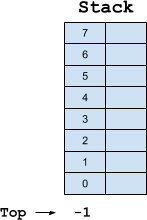
\includegraphics[scale=.35]{images/stack_intro_01.png} & 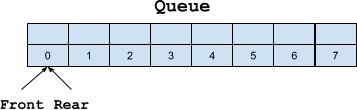
\includegraphics[scale=.35]{images/queue_intro_01.png}\\
    & \texttt{Initial State} & \texttt{Initial State} \\
    \hline
    \textbf{Push 7} & 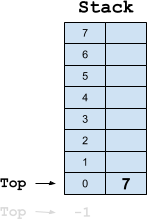
\includegraphics[scale=.35]{images/stack_intro_02.png} & 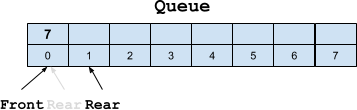
\includegraphics[scale=.35]{images/queue_intro_02.png} \\
    & 
    \begin{minipage}[l]{6cm}
    \texttt{1. Increment Top} \\
    \texttt{2. Insert item at Top}\\
    \end{minipage}
    & 
    \begin{minipage}[l]{6cm}
    \vspace{5mm}
    \texttt{1. Insert item at Rear} \\
    \texttt{2. Increment Rear}\\
    \end{minipage}\\
    \hline
    \textbf{Push 11} & 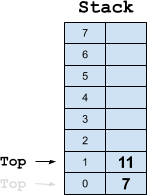
\includegraphics[scale=.35]{images/stack_intro_03.png} & 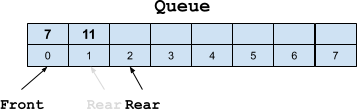
\includegraphics[scale=.35]{images/queue_intro_03.png} \\
    & 
    \begin{minipage}[l]{6cm}
    \texttt{1. Increment Top} \\
    \texttt{2. Insert item at Top}\\
    \end{minipage}\\
    & 
    \begin{minipage}[l]{6cm}
    \vspace{5mm}
    \texttt{1. Insert item at Rear} \\
    \texttt{2. Increment Rear}\\
    \end{minipage}\\
    \hline
    \textbf{Push 13,5,2}  & 
    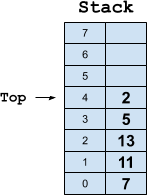
\includegraphics[scale=.35]{images/stack_intro_04.png} & 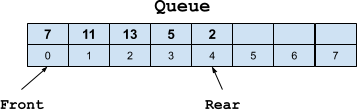
\includegraphics[scale=.35]{images/queue_intro_04.png} \\
    &
    \begin{minipage}[l]{6cm}
    \texttt{Resulting Stack After 13,5,2 are pushed} 
    \end{minipage}\\
    & 
    \begin{minipage}[l]{6cm}
    \vspace{5mm}
    \texttt{Resulting Queue After 13,5,2 are pushed} 
    \end{minipage}\\
    \hline 
    \caption{Stack Queue Example Inserts}
    \label{table:visible_stack_queue_add}
\end{longtable}

The resulting data structures are identical after inserting 5 values into each. The values are in the same order. They are using the same type of container (an array), and they have the same types of operations (Push, Pop). The main difference between the two is in how each algorithm implements the  "removal" method. Stacks remove from the "top" and queues remove from the "front", entirely changing the order in which they operate. But is that true? Below we remove an item from each, and yes, we get a 2 from the stack, and a 7 from the queue. But does the subtle differences in each algorithm make these structures really that different?

\begin{longtable}{|M{2cm}|M{6cm}|M{6cm}|}
    \hline
    \textbf{Pop} & 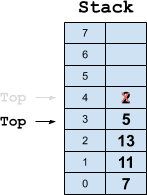
\includegraphics[scale=.35]{images/stack_intro_05.png} & 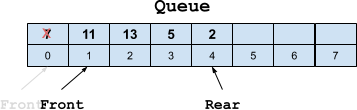
\includegraphics[scale=.35]{images/queue_intro_05.png} \\
    & 
    \begin{minipage}[l]{6cm}
    \texttt{1. Copy value at Top (2)} \\
    \texttt{2. Decrement Top}\\
    \texttt{3. Return value 2}\\
    \end{minipage}\\
    & 
    \begin{minipage}[l]{6cm}
    \vspace{5mm}
    \texttt{1. Copy value at Front (7)} \\
    \texttt{2. Increment Front}\\
    \texttt{3. Return value 7}\\
    \end{minipage}\\
    \hline 
    \textbf{Pop} & 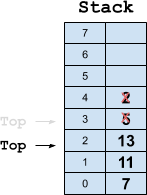
\includegraphics[scale=.35]{images/stack_intro_06.png} & 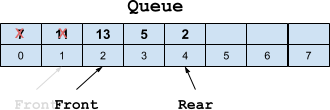
\includegraphics[scale=.35]{images/queue_intro_06.png} \\
    & 
    \begin{minipage}[l]{6cm}
    \texttt{1. Copy value at Top (5)} \\
    \texttt{2. Decrement Top}\\
    \texttt{3. Return value 5}\\
    \end{minipage}\\
    & 
    \begin{minipage}[l]{6cm}
    \vspace{5mm}
    \texttt{1. Copy value at Front (11)} \\
    \texttt{2. Increment Front}\\
    \texttt{3. Return value 11}\\
    \end{minipage}\\
    \hline 
    \caption{Stack Queue Example Removals}
    \label{table:visible_stack_queue_remove}
\end{longtable}

Try mixing up the operations performed by doing pushes and pops randomly\footnote{I didn't do this because I didn't want to have a 4 page example}. Our containers would have been extremely different in that scenario. In fact you should do this as an exercise to make sure you understand how both data structures work.\\

I hope that I have shown you that a "data structure" coupled with an "algorithm" become partners in creating "advanced structures". It is a little stretch to call a stack or a queue an "advanced structure", but as introductory examples, they work fine. They showed us that a "data structure" stores data and an "algorithm" unambiguously controlled how that data was stored. Now all we need to do is use more complex algorithms to control how data the data is stored and retrieved, and we will be solving cool complex problems\footnote{Also known as "Advanced Structures \& Algorithms"}.\\

\mysubsection{Course Content Overview}

Linear Data Structure: Linked List, Stack, Queue, Array.
Hierarchical data structures: Tree, Heap, Trie.
Other Data Structures: Hash, Graph, Matrix.

A data structure is a data organization, management, and storage format that enables efficient access and modification.
Most of the problems in computer science have some sort of data associated with, using which we have to solve the problem or we have to come up with a sort of conclusion.
So, as the above line states, the data structure is a way to organize and manage that data at memory level such that we can effectively and efficiently do operation on that data. Here, operations on data are like accessing, modifying or maybe deleting that data.
In other words, we have to structure and organize the raw data available for the problem statement, such that we can efficiently perform the required operation to solve the problem.
More precisely, a data structure is a collection of data values, the relationships among them, and the functions or operations that can be applied to the data.
Generally, developers know that Data structure is just an organization and management of data but it’s more than that and that’s why Wikipedia has added the above line in the definition. This statement is equally important to understand the role of data structure.
Here, in this statement the most useful words are “… the functions or operations that can be applied to the data”. If you don’t have much knowledge yet about actual data structures(Linked List, Stack, Queue, etc.), then it is very difficult to understand this line of definition.
In layman’s language, we can say that many data structures have the same organization of data at the memory level but they can provide the different functions and operations on them which differentiate with each other.
Let me give an example of the same. Stack and Queue can be implemented using Linked List have the same data organization at the memory level but they are providing different functions that are useful in different scenarios. Like, Queue can be used for First in first out(FIFO) scenarios while Stack can be used in Last in first out(LIFO) scenarios.
Few examples of Data Structures
Linear Data Structure: Linked List, Stack, Queue, Array.
Hierarchical data structures: Tree, Heap, Trie.
Other Data Structures: HashMap, Graph, Matrix.
Note: If you are a beginner and don’t know much about Queues or Stacks or LinkedList, don’t worry. You can follow me for my upcoming series on “Data Structures for beginners with the real-world application”.
Algorithms
An algorithm is a finite sequence of well-defined, computer-implementable instructions, typically to solve a class of problems or to perform a computation. Algorithms are unambiguous specifications for performing calculation, data processing, automated reasoning, and other tasks. - Wikipedia

I can understand that as a beginner you may be confused after reading this definition. Let’s understand this in layman’s language first and then jump to the technical definition of Algorithm.
In the simplest words, Algorithm is nothing but a sequence of steps to be followed to solve any problem or to achieve the desired output.
By taking this simplest definition now in your mind, let's understand the words mentioned in Wikipedia’s definition.
Finite sequence: The number of steps to solve a problem should be finite in numbers.
Well-defined: There should not be any ambiguity in any step.
Computer-implementable instructions: As we are talking about Computer Science related problems here, the steps should be understood by the computer.
A class of problems: Set of problems that have the same end goal or may have the same sequence of steps to reach the desired output.
Now let me put this down in one sentence.
An algorithm is a process of finite well-defined steps to be carried out to solve a particular class of problems or to get the desired output.
Few examples of Algorithms
Sorting Algorithms: Merge Sort, Quick Sort, Tim Sort, etc.
Searching Algorithms: Linear Search, Binary Search.
Shortest Path Algorithms: Dijkstra’s algorithm, Bellman-Ford algorithm.
Summing-up
Data Structure is about organising and managing data effectively such that we can perform specific operation efficiently, while Algorithm is a step-by-step procedure to be followed to reach the desired output.
To understand the Data Structure in a meaningful way, you also have to consider the understanding of memory allocation as well as space and time complexity to perform a specific operation on it.
We have to note that, different Data Structures can use the same internal memory management and organisation but they can differ by the functions they are providing which can be used to solve a specific class of problems. (Read the “Data Structures” Chapter).
Steps in an algorithm can use one or many data structure(s) to solve a problem.
One algorithm can internally use separate Data Structure to solve the same problem but that may lead to varying in performance. Ex. A Graph algorithm can use Adjacency List or Matrix representation of Graph for solving a problem but their Time Complexity and Space Complexity will be vary based on choices of the Data Structure.

\newpage
\mysection{Commenting Code}

Comments are important! In academia, you think your professors are just trying to punish you, but we are giving you wisdom that we acquired. Un-commented programs are hard to read, even if written in your own hand. But let me give you a few more reasons to motivate you. 1) In industry, your comments will allow another programmer to read and understand your code much faster, besides the fact that poorly commented code will probably \textbf{get rejected} anyway by whatever system your company uses to manage versions or continuous integration. 2) Another factor is that since you have to post your code on Github, you want to put your best face forward when making your code publicly visible. Putting many well commented working programs on your Github repository will look good when you are applying for jobs. 3) Your grade in this course. I'll leave it at that, so, you might as well start commenting your code.\\


\mysubsection{Commenting Extremes}

The amount and style of comments is an entire subject that is debated to this day, and depending on the task (or workplace), you would vary the amount and style of your comments. Some extremes are: 1. no comments at all (competitive programming), 2. self documenting and 3. industry requirements. 

\mysubsubsection{Competitive Programming}

In competitive programming, you use short variable names, and short cryptic snippets of code that run fast with no need for an explanation. Why? It's all about a speedy solution at a competition. Comments are almost in the way. The only time you would use comments is when you write solutions to be studied for later. Other than that, there is no need to use descriptive variable names, or comments to explain what a code block is doing since the code is never really meant to be read again at a later date. Here is an example of competitive programming code. Its not totally devoid of hints as to what its doing, but I think we can agree that it's not awesomely clear.

\begin{minted}[]{c++}
typedef pair<int, int> ii;
typedef vector<ii> vii;
typedef vector<int> vi;
vi dfs_num;
void dfs(int u)
{
    dfs_num[u] = VISITED;
    for (int j = 0; j < (int)AdjList[u].size(); j++)
    {
        ii v = AdjList[u][j];
        if (dfs_num[v.first] == UNVISITED)
            dfs(v.first);
    }
}
\end{minted}

 \mysubsubsection{Self Documenting}
 
 In case you don't remember, "self documenting" code is \textit{using naming conventions in place of explicit comments to make the logic of the code more obvious to human readers}. This really means that you name functions and variable names in such a way that a human reader can understand the code by just reading the code. In other words, use long descriptive variable names and function names. Below is an example of self documenting code \cite{wiki:selfdoc}. 

\begin{minted}[]{c++}
size_t count_alphabetic_chars(const char *text)
{
    if (text == NULL)
        return 0;

    size_t  count = 0;

    while (*text != '\0')
    {
        if (is_alphabetic(*text))
            count++;
        text++;
    }

    return count;
}
\end{minted}

\mysubsubsection{Industry}

 Industry will have the most stringent requirements dealing with comments. In fact my remark about code being "rejected" at the beginning of this section is not an exaggeration, its a common practice. One reason companies have strict rules about comments is because they use software to "auto generate" documentation. Auto doc generation mostly deals with class, method, or function comment blocks, but they will also have rules on other things like inline comments and variable names. With inline comments, they mostly scan to see what percentage of lines have a comment to make sure there are an adequate number of comments. With variable names, some companies require you to name variables in very specific ways: \textit{int\_score} or \textit{string\_name} so it's easy to identify a variable type when seeing it in code. This just scratches the surface dealing with the amount and types of rules that could be put in place dealing with comments. 
 
 \mysubsection{Not Formatting}
 
 The major goal of this section is about adding appropriate comments to your source code. It is not about formatting your code. If I started slapping down rules on formatting, it would open up a whole new world of crazy. If there are many opinions on the "right way" to add comments, there are even more opinions on the "right way" of formatting code. Just like the two camps for parenthesis: do you put curly braces on their own line? Or do you put curly braces on the same line?\\
 
 \begin{center}
 \begin{tabular}{| c | c |}
 \hline
    
\includegraphics[scale=.6]{images/curly_braces_2.png} &  
\includegraphics[scale=.6]{images/curly_braces_1.png}\\
     \tiny{Same Line} & \tiny{Own Line}\\
     \hline
 \end{tabular}
 \end{center}

And what about how to format variable names and function names:


 \begin{center}
 \begin{tabular}{| c | c | c | c | }
 \hline
    \ccb{camelCase} &  \ccb{PascalCase} & \ccb{snake\_case}  & \ccb{kebab-case}\footnote{Some languages allow the "dash" in variable names}\\
    \hline
 \end{tabular}
 \end{center}

Don't forget the mixing of rules either: "capitalize method names but not function names" and "use snake\_case for params, but not for function names", and on and on it goes. There are many many "styles" or "guides" on how to format your code. If you are interested in standardizing your programs and your own style, here is Googles \href{https://google.github.io/styleguide/cppguide.html}{style guide} for C++.

\mysubsection{Comments For Assignments}

The previous few sections are there to show you that I'm not being crazy with my expectations on comments, because there is a \textbf{whole world of crazy} when it comes to styling code. In general, my rules for comments are somewhere in between competitive programming and industry. I will give examples in the following sections, but here are my basic rules for comments: \\

\begin{enumerate}
    \item Programs get a comment block at the top ALWAYS.
    \item Functions and Classes get a comment block ALWAYS.
    \item Line up your comments!
    \item Put variable declarations on a single line and at the beginning of a code block, so you can comment each of them if needed.
    \item Place comments throughout your code giving near English explanations of your code's logic.
\end{enumerate}


\mysubsubsection{Commenting Variables}

Let's start with how I would like you to comment your variables in your code. Always place your variables at the top of the code block, on separate lines. This allows you to write a comment for each variable on its own line. Remember to line up your comments. \\
\textbf{Good}\\
\begin{minted}[]{c++}
  int num1;                 // 3 vars for users entering numbers
  int num2;
  int num3;     
  double average;           // calculated average of entered numbers
  int score1;               // score on exam 1
  int score2;               // score on exam 2
\end{minted}

\begin{minted}[]{c++}
    T **Array;          // Templated pointer to dynamic array
    int Next;           // Next available location in heap array
    int MaxSize;        // Max array size
    int HeapSize;       // Actual number of items in the array.
    bool isMax;         // true = max heap, false = min heap
\end{minted}

\textbf{Bad}\\
\begin{minted}[]{c++}
  // user  nums
  int num1, num2, num3;          
  double average;    //avg nums
  int score1,    //score exam
      score2;			    // score exam
\end{minted}

\mysubsubsection{Comment Blocks}

A comment block at the beginning of your program, a function, or a method will use the following style. VSCode has plugins to auto generate blocks for you. 

\begin{minted}[]{c++}
/**
*
* 
*
*/
\end{minted}

OR

\begin{minted}[]{c++}
/*****************************************************************************
*
* 
*
*****************************************************************************/
\end{minted}


\mysubsubsection{Program Comment Block}

The number of asterisks on the top and bottom line only matter if your writing a comment block for your program like below. The longer lines of asterisks helps create a nice visual distinction separating it from the rest of the program.\\

\textbf{Program Comment Template}\\

\begin{minted}[]{c++}
/*****************************************************************************
*                    
*  Author:           (your name)
*  Email:            (your email address)
*  Label:            (program's label from assignment list)
*  Title:            (short title from assignment, if any)
*  Course:           (course number and prefix)
*  Semester:         (semester and year)
* 
*  Description:
*        describe program here thoroughly 
* 
*  Usage:
*        how to use the program if necessary
* 
*  Files:            (list of all source files used in this program)
*****************************************************************************/
\end{minted}

\textbf{Program Comment Example}\\

\begin{minted}[]{c++}
/*****************************************************************************
*                    
*  Author:           Terry Griffin
*  Email:            terry.griffin@msutexas.edu
*  Label:            A04
*  Title:            Linked List Class
*  Course:           CMPS 3013
*  Semester:         Spring 2020
* 
*  Description:
*        This program implements a class that allows a linked list to be used just like 
*        an array. It overloads the "[]" (square brackets) to simulate accessing seperate 
*        array elements, but really it traverses the list to find the specified node using
*        an index value. It also overloads the "+" and "-" signs allowing a user to "add"
*        or "push" items onto the end of the list, as well as "pop" items off the end of our 
*        array. This class is not meant to replace the STL vector library, its simply a project
*        to introduce the beginnings of creating complex / abstract data types. 
*        
*  Usage: 
*       - $ ./main filename
*       - This will read in a file containing whatever values to be read into our list/array. 
*       
*  Files:            
*       main.cpp    : driver program 
*       list.h      : header file with list defintion
*       list.cpp    : list implementation
*****************************************************************************/
\end{minted}

\mysubsubsection{Class Comment}

\textbf{Class Comment Template}\\

\begin{minted}[]{c++}
/**
 * Class Name
 * 
 * Description:
 *      Description of your class and what it does
 * 
 * Public Methods:
 *      - A list of 
 *      - each public method
 *      - with return types
 * 
 * Private Methods:
 *      - A list of 
 *      - each private method
 *      - with return types
 * 
 * Usage: 
 * 
 *      - examples of how
 *      - to use your class 
 *      
 */
\end{minted}

\textbf{Class Comment Example}

\begin{minted}[]{c++}
/**
 * Huffman
 * 
 * Description:
 *      This class implements a compressions algorithm called Huffman Coding.
 *      Huffman coding assigns codes to characters such that the length of the 
 *      code depends on the relative frequency or weight of the corresponding 
 *      character. Huffman codes are of variable-length, and prefix-free
 * 
 * Public Methods:
 *                          Huffman()                               
 *      void                BuildFrequencyTable(string filename)
 *      string              LookupCode(char key)
 *      void                Analyze()
 *      map<char, string>   GetCodes()
 * 
 * Private Methods:
 *      void                _BuildLookupTable
 *      void                _BuildTree
 *      int                 _maxDepth
 * 
 * Usage: 
 * 
 *      Huffman H(filename):                        // Create Instance of Huffman
 *                                                  // and build freq table. 
 *      H.GetCodes();                               // get map <char,string> of codes
 * 
 *                                                  // or
 *      
 *      Huffman H;                                  // do seperately
 *      H.BuildFrequencyTable(filename);            // or use to re-build another file
 *      H.LookupCode('s')                           // get code for 's' 
 *      
 */
\end{minted}

\mysubsubsection{Function Comment}

\textbf{Function Comment Template}\\
\begin{minted}[]{c++}
    /**
     * Public/Private/Protected : function_name
     * 
     * Description:
     *      Describe the functions purpose
     * 
     * Params:
     *      - list params
     *      - one per line
     *      - with return type
     *      - and one line description
     * 
     * Returns:
     *      - what does this function return (including the type)?
     */
\end{minted}

\textbf{Function Comment Example}

\begin{minted}[]{c++}
    /**
     * Public : LoadList
     * 
     * Description:
     *      Loads an array of integers into a linked list.
     * 
     * Params:
     *      [int*]    :  array of integers
     *      [int]     :  array size
     * 
     * Returns:
     *      [type] List*   : a pointer to a linked list of integers.
     */
\end{minted}

\mysubsubsection{Code Comment Example}

\begin{itemize}
    \item Code should be commented enough to describe what is being done in general, or to clarify possibly confusing lines of code.
    \item The following is taken from a "heap" class. Knowing in general how a heap works, and by having access to the other code in the file, the comments below are enough to give the reviewer an idea of what this function is doing. 
    \item Notice that not all the comments line up, or use a single "style". I just request that your comments be consistent and neat. I chose to put some lined up to the far right, and some lined up towards the left. It's a bit of a contrived example, but I wanted to show I would accept multiple styles. 
    \item The one little pet peeve I have is that you place a space between the comment and the single line comment.
    \begin{itemize}
        \item Good: $//\;\;$This is a good comment with space after slashes.
        \item Bad: $//$This is a bad comment. No space!
    \end{itemize}
\end{itemize}

\textbf{Inline Code Comment Example}\\
\begin{minted}[]{c++}
    /**
     * public : PickChild:
     *      Return index of child to swap with or -1 to not swap.
     * 
     * Params:
     *      [int] index - index of parent element
     * 
     * Returns
     *      [int] index - index to swap with or -1 to not swap
     */
    int PickChild(int i) {
        if (RightChild(i) >= Next) {        // No right child
            if (LeftChild(i) >= Next) {     // No left child
                return -1;              
            } else {                        // There there is only a left child
                return LeftChild(i);
            }
        } else {                            // The right child exists 
            if(isMax){  
                // This is a "maxheap"
                // return child with "greater" value
                if (Array[RightChild(i)]->priority > Array[LeftChild(i)]->priority) {
                    return RightChild(i);
                } else {
                    return LeftChild(i);
                }
            }else{
                // return child with "smaller" value
                if (Array[RightChild(i)]->priority < Array[LeftChild(i)]->priority) {
                    return RightChild(i);
                } else {
                    return LeftChild(i);
                }   
            }

        }
    }
\end{minted}

\newpage
\mysection{Linked Lists}

\begin{figure}[h]
 \centering
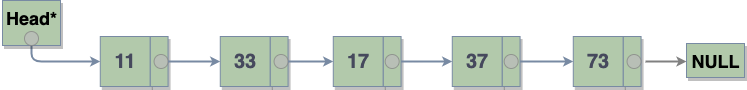
\includegraphics[scale=.40]{images/singly_linked_list.png}
\end{figure}

\mysubsection{Linked Lists in General}

A linked list as a linear collection of data elements whose order is not a contiguous set of memory locations like an array, and who's order is not determined by their actual (physical) location in memory. The order is determined by one element containing the address to the next element in the list. This means nodes in a linked list could be stored in an order that is nothing like we visualize a list as being. The above image is the typical representation of a linked list that abstracts out all of the "address" information. The following image is a similar representation, but showing actual addresses for each node (as well as the address for head).\\

At a minimum, each node contains some data element and a reference (pointer) to the next element in the list. A list can be ordered or unordered depending on needs of implementation. But, one inherent attribute of a linked list is the efficient insertion and deletion of nodes at any an all positions. The structure grows and shrinks with each addition or deletion. One drawback that lists have is the need to access them linearly. When compared to arrays, accessing elements directly (aka random access) is not possible. Another advantage of arrays is they have better cache locality\supcite{Locality63}. \\

A linked list whose nodes contain two fields: an integer value and a link to the next node. The last node is linked to a terminator used to signify the end of the list. Linked lists are among the simplest and most common data structures. They can be used to implement several other common abstract data types, including lists, stacks, queues, associative arrays, and S-expressions, though it is not uncommon to implement those data structures directly without using a linked list as the basis.\\

The principal benefit of a linked list over a conventional array is that the list elements can be easily inserted or removed without reallocation or reorganization of the entire structure because the data items need not be stored contiguously in memory or on disk, while restructuring an array at run-time is a much more expensive operation. Linked lists allow insertion and removal of nodes at any point in the list, and allow doing so with a constant number of operations by keeping the link previous to the link being added or removed in memory during list traversal.\\

On the other hand, since simple linked lists by themselves do not allow random access to the data or any form of efficient indexing, many basic operations—such as obtaining the last node of the list, finding a node that contains a given datum, or locating the place where a new node should be inserted—may require iterating through most or all of the list elements. The advantages and disadvantages of using linked lists are given below. Linked list are dynamic, so the length of list can increase or decrease as necessary. Each node does not necessarily follow the previous one physically in the memory.\\


\begin{minted}[]{c++}
void PrintList(){
    if(!Head){
        cout<<"Empty"<<endl;
        return;
    }else{
        cout<<"The sizeof `Node` in bytes is: "<<sizeof(Head->Data)<<endl;
        cout<<"Address of `Head` is: "<<&Head<<endl;
        cout<<"`Head` points to ->"<<Head<<endl<<endl;
    
        Node *Temp = Head;
        while(Temp != NULL){
            cout<<"|Address: "<<Temp<<" |Data: "<<Temp->Data<<" |Next: "<<Temp->Next<<" | "<<" -> "<<endl;
            Temp = Temp->Next;
        }
        cout<<"NULL"<<endl<<endl;
    }
}
\end{minted}

\textbf{Output:}

\begin{verbatim}
The sizeof `Node` in bytes is: 4
Address of `Head` is: 0x7ffeeeafd550
`Head` points to ->0x7faaf3c05920

|Address: 0x7faaf3c05920 |Data: 1 |Next: 0x7faaf3c05910 |  -> 
|Address: 0x7faaf3c05910 |Data: 56 |Next: 0x7faaf3c05900 |  -> 
|Address: 0x7faaf3c05900 |Data: 20 |Next: 0x7faaf3c058f0 |  -> 
|Address: 0x7faaf3c058f0 |Data: 39 |Next: 0x7faaf3c058e0 |  -> 
|Address: 0x7faaf3c058e0 |Data: 20 |Next: 0x7faaf3c058d0 |  -> 
|Address: 0x7faaf3c058d0 |Data: 56 |Next: 0x0 |  -> NULL
\end{verbatim}

\begin{minted}[]{c++}
struct Node {
    Person Data;
    Node *Next;
    Node(Person p) {
        Data = p;
        Next = NULL;
    }
};

struct Person {
    string Name;
    int Age;
    Person() {
        Name = "";
        Age = 0;
    }
    Person(string n, int a) {
        Name = n;
        Age = a;
    }
};

void Print() {
    Node *Current = Head;
    cout << sizeof(Current->Data) << endl;
    while (Current) {
        cout << "|" << Current->Data.Name << "|" << Current << " ->\n";
        cout ;
        Current = Current->Next;
    }
    cout << "NULL" << endl;
}
\end{minted}

\textbf{Output:}

\begin{verbatim}
40
|Abby|0x8d2200| -> 
|Chuck|0x8d2240| -> 
|Daphne|0x8d23c0| -> 
|Donnie|0x8d2280| -> 
|Echo|0x8d22c0| -> 
|Gerald|0x8d2380| -> 
|MarkyMark|0x8d2300| -> NULL
\end{verbatim}

\mysubsection{Singly Linked Lists}

\begin{center}
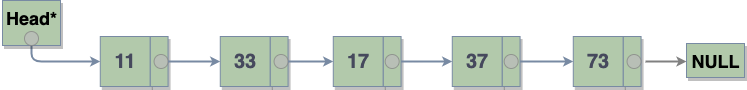
\includegraphics[scale=.40]{images/singly_linked_list.png}
\end{center}

\mysubsection{Circular Linked Lists}
\begin{center}
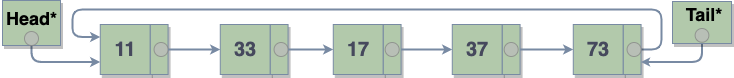
\includegraphics[scale=.40]{images/singly_linked_list_circular.png}
\end{center}


\mysubsection{Doubly Linked Lists}

\begin{center}
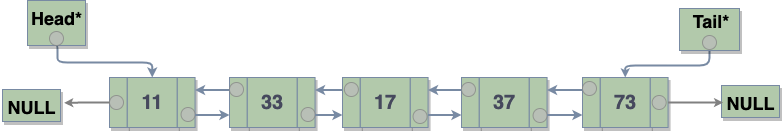
\includegraphics[scale=.40]{images/doubly_linked_list.png}
\end{center}


\mysubsection{Circular Doubly Linked Lists}

\begin{center}
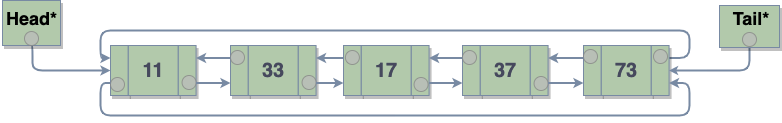
\includegraphics[scale=.40]{images/linked_list_double_circular.png}
\end{center}


\newpage
\hypertarget{body-content}{}
\hypertarget{introduction-to-data-structures-and-algorithms}{%
	\mysection{Introduction to Data Structures and
		Algorithms}\label{introduction-to-data-structures-and-algorithms}}

Data Structure is a way of collecting and organising data in such a way
that we can perform operations on these data in an effective way. Data
Structures is about rendering data elements in terms of some
relationship, for better organization and storage. For example, we have
some data which has, player's \textbf{name} "Virat" and \textbf{age} 26.
Here "Virat" is of \textbf{String} data type and 26 is of
\textbf{integer} data type.

We can organize this data as a record like \textbf{Player} record, which
will have both player's name and age in it. Now we can collect and store
player's records in a file or database as a data structure. \textbf{For
example}: "Dhoni" 30, "Gambhir" 31, "Sehwag" 33

If you are aware of Object Oriented programming concepts, then a
\texttt{class} also does the same thing, it collects different type of
data under one single entity. The only difference being, data structures
provides for techniques to access and manipulate data efficiently.

In simple language, Data Structures are structures programmed to store
ordered data, so that various operations can be performed on it easily.
It represents the knowledge of data to be organized in memory. It should
be designed and implemented in such a way that it reduces the complexity
and increases the efficiency.

\begin{center}\rule{0.5\linewidth}{0.5pt}\end{center}

\hypertarget{basic-types-of-data-structures}{%
	\mysubsection{Basic types of Data
		Structures}\label{basic-types-of-data-structures}}

As we have discussed above, anything that can store data can be called
as a data structure, hence Integer, Float, Boolean, Char etc, all are
data structures. They are known as \textbf{Primitive Data Structures}.\\

Then we also have some complex Data Structures, which are used to store
large and connected data. Some example of \textbf{Abstract Data
Structure} are :

\begin{itemize}
	\tightlist
	\item
	      Linked List
	\item
	      Tree
	\item
	      Graph
	\item
	      Stack, Queue etc.
\end{itemize}

All these data structures allow us to perform different operations on
data. We select these data structures based on which type of operation
is required. We will look into these data structures in more details in
our later lessons.

\begin{figure}
    \centering
    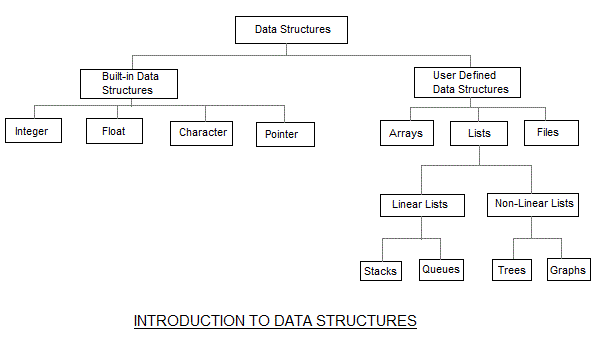
\includegraphics[scale=.5]{images/introduction-to-data-structures.png}
    \caption{Caption}
    \label{fig:my_label}
\end{figure}


\hfill\break

The data structures can also be classified on the basis of the following
characteristics:

\begin{table}
\begin{tabular}{|p{.20\textwidth}|p{.8\textwidth}|}
	\hline
	\textbf{Characteristic}   & \textbf{Description}\\                    
	\hline
	Linear          & In Linear data structures,the data items are arranged in a linear sequence. Example: \textbf{Array}\\
	\hline
	Non-Linear      & In Non-Linear data structures,the data items are not in sequence. Example: \textbf{Tree}, \textbf{Graph}\\
	\hline
	Homogeneous     & In homogeneous data structures,all the elements are of same type. Example: \textbf{Array}\\
	\hline
	Non-Homogeneous & In Non-Homogeneous data structure, the elements may or may not be of the same type. Example: \textbf{Structures}\\
	\hline
	Static          & Static data structures are those whose sizes and structures associated memory locations are fixed, at compile time. Example:\textbf{Array}\\
	\hline
	Dynamic         & Dynamic structures are those which expands or shrinks depending upon the program need and its execution. Also, their associated memory locations changes. Example: \textbf{Linked List created using pointers}\\
	\hline
\end{tabular}
\end{table}
\begin{center}\rule{0.5\linewidth}{0.5pt}\end{center}

\hypertarget{what-is-an-algorithm}{%
	\mysubsection{What is an Algorithm ?}\label{what-is-an-algorithm}}

An algorithm is a finite set of instructions or logic, written in order, to accomplish a certain predefined task. Algorithm is not the complete code or program, it is just the core logic(solution) of a problem, which can be expressed either as an informal high level description as \textbf{pseudocode} or using a \textbf{flowchart}.\\

Every Algorithm must satisfy the following properties:

\begin{enumerate}
	\tightlist
	\item
	      \textbf{Input}- There should be 0 or more inputs supplied externally
	      to the algorithm.
	\item
	      \textbf{Output}- There should be atleast 1 output obtained.
	\item
	      \textbf{Definiteness}- Every step of the algorithm should be clear and
	      well defined.
	\item
	      \textbf{Finiteness}- The algorithm should have finite number of steps.
	\item
	      \textbf{Correctness}- Every step of the algorithm must generate a
	      correct output.
\end{enumerate}

An algorithm is said to be efficient and fast, if it takes less time to execute and consumes less memory space. The performance of an algorithm is measured on the basis of following properties :

\begin{enumerate}
	\tightlist
	\item
	      Time Complexity
	\item
	      Space Complexity
\end{enumerate}

\begin{center}\rule{0.5\linewidth}{0.5pt}\end{center}

\hypertarget{space-complexity}{%
	\mysubsection{Space Complexity}\label{space-complexity}}

Its the amount of memory space required by the algorithm, during the course of its execution. Space complexity must be taken seriously for multi-user systems and in situations where limited memory is available.\\

An algorithm generally requires space for following components :

\begin{itemize}
	\tightlist
	\item
	      \textbf{Instruction Space:} Its the space required to store the
	      executable version of the program. This space is fixed, but varies
	      depending upon the number of lines of code in the program.
	\item
	      \textbf{Data Space:} Its the space required to store all the constants
	      and variables(including temporary variables) value.
	\item
	      \textbf{Environment Space:} Its the space required to store the
	      environment information needed to resume the suspended function.
\end{itemize}


\hypertarget{time-complexity}{%
	\mysubsection{Time Complexity}\label{time-complexity}}

Time Complexity is a way to represent the amount of time required by the program to run till its completion. It's generally a good practice to try to keep the time required minimum, so that our algorithm completes it's execution in the minimum time possible. 

\hypertarget{body-content}{}
\hypertarget{space-complexity-of-algorithms}{%
\section{Space Complexity of
Algorithms}\label{space-complexity-of-algorithms}}

Whenever a solution to a problem is written some memory is required to
complete. For any algorithm memory may be used for the following:

\begin{enumerate}
\tightlist
\item
  Variables (This include the constant values, temporary values)
\item
  Program Instruction
\item
  Execution
\end{enumerate}

\begin{quote}
\emph{\textbf{Space complexity} is the amount of memory used by the
algorithm (including the input values to the algorithm) to execute and
produce the result.}
\end{quote}

Sometime \textbf{Auxiliary Space} is confused with Space Complexity. But
Auxiliary Space is the extra space or the temporary space used by the
algorithm during it's execution.

\textbf{Space Complexity} = \textbf{Auxiliary Space + Input space}

\begin{center}\rule{0.5\linewidth}{0.5pt}\end{center}

\hypertarget{memory-usage-while-execution}{%
\mysubsection{Memory Usage while Execution}\label{memory-usage-while-execution}}

While executing, algorithm uses memory space for three reasons:

\begin{enumerate}
\item
  \textbf{Instruction Space}

  It's the amount of memory used to save the compiled version of
  instructions.
\item
  \textbf{Environmental Stack}

  Sometimes an algorithm(function) may be called inside another
  algorithm(function). In such a situation, the current variables are
  pushed onto the system stack, where they wait for further execution
  and then the call to the inside algorithm(function) is made.

  For example, If a function \texttt{A()} calls function \texttt{B()}
  inside it, then all th variables of the function \texttt{A()} will get
  stored on the system stack temporarily, while the function
  \texttt{B()} is called and executed inside the funciton \texttt{A()}.
\item
  \textbf{Data Space}

  Amount of space used by the variables and constants.
\end{enumerate}

But while calculating the \textbf{Space Complexity} of any algorithm, we usually consider only \textbf{Data Space} and we neglect the \textbf{Instruction Space} and \textbf{Environmental Stack}.

\begin{center}\rule{0.5\linewidth}{0.5pt}\end{center}

\hypertarget{calculating-the-space-complexity}{%
\mysubsection{Calculating the Space
Complexity}\label{calculating-the-space-complexity}}

For calculating the space complexity, we need to know the value of
memory used by different type of datatype variables, which generally
varies for different operating systems, but the method for calculating
the space complexity remains the same.

\begin{longtable}[]{@{}ll@{}}
\toprule
Type & Size\tabularnewline
\midrule
\endhead
bool, char, unsigned char, signed char, \_\_int8 & 1 byte\tabularnewline
\_\_int16, short, unsigned short, wchar\_t, \_\_wchar\_t & 2
bytes\tabularnewline
float, \_\_int32, int, unsigned int, long, unsigned long & 4
bytes\tabularnewline
double, \_\_int64, long double, long long & 8 bytes\tabularnewline
\bottomrule
\end{longtable}

\hfill\break

Now let's learn how to compute space complexity by taking a few
examples:

\begin{minted}[]
{
    int z = a + b + c;
    return(z);
}
\end{minted}

In the above expression, variables \texttt{a}, \texttt{b}, \texttt{c}
and \texttt{z} are all integer types, hence they will take up 4 bytes
each, so total memory requirement will be
\texttt{(4(4)\ +\ 4)\ =\ 20\ bytes}, this additional 4 bytes is for
\textbf{return value}. And because this space requirement is fixed for
the above example, hence it is called \textbf{Constant Space
Complexity}.

Let's have another example, this time a bit complex one,

\begin{minted}[]
// n is the length of array a[]
int sum(int a[], int n)
{
    int x = 0;     // 4 bytes for x
    for(int i = 0; i < n; i++)  // 4 bytes for i
    {    
        x  = x + a[i];     
    }
    return(x);
}
\end{minted}

\begin{itemize}
\tightlist
\item
  In the above code, \texttt{4*n} bytes of space is required for the
  array \texttt{a{[}{]}} elements.
\item
  4 bytes each for \texttt{x}, \texttt{n}, \texttt{i} and the return
  value.
\end{itemize}

Hence the total memory requirement will be \texttt{(4n\ +\ 12)}, which is increasing linearly with the increase in the input value \texttt{n}, hence it is called as \textbf{Linear Space Complexity.}

Similarly, we can have quadratic and other complex space complexity as well, as the complexity of an algorithm increases.

But we should always focus on writing algorithm code in such a way that we keep the space complexity \textbf{minimum}.




\newpage
\section{Pointers}
\label{sec:pointers}

In C++, pointers are variables that store the memory addresses of other variables.

\hypertarget{address}{%
\subsection{Addresses in C++}\label{address}}

If we have a variable \texttt{var} in our program, \texttt{\&var} will give us its address in the memory.\\
\vspace{.5cm}

For example,

\begin{minted}[]{c++}
#include <iostream>
using namespace std;

int main()
{
    // declare variables
    int var1 = 3;
    int var2 = 24;
    int var3 = 17;

    // print address of var1
    cout << "Address of var1: "<< &var1 << endl;

    // print address of var2
    cout << "Address of var2: " << &var2 << endl;

    // print address of var3
    cout << "Address of var3: " << &var3 << endl;
}
\end{minted}

\textbf{Output}

\begin{minted}[bgcolor=bg]{text}
Address of var1: 0x7fff5fbff8ac
Address of var2: 0x7fff5fbff8a8
Address of var3: 0x7fff5fbff8a4
\end{minted}

Here, \texttt{0x} at the beginning represents the address is in the hexadecimal form. Notice that the first address differs from the second by 4 bytes and the second address differs from the third by 4 bytes. This is because the size of an \texttt{int} variable is 4 bytes in a 64-bit system.\\

\textbf{Note:} You may not get the same results when you run the program.

% \doublelinewithspace{.0cm}

\doublelinewithspace{.0cm}

\hypertarget{pointer-variable}{%
\subsection{C++ Pointers}\label{pointer-variable}}

As mentioned above, pointers are used to store addresses rather than
values.

Here is how we can declare pointers.

\begin{minted}[]{c++}
int *pointVar;
\end{minted}

Here, we have declared a pointer \texttt{pointVar} of the \texttt{int} type. We can also declare pointers in the following way.

\begin{minted}[]{c++}
int* pointVar; // preferred syntax
\end{minted}

Let's take another example of declaring pointers.

\begin{minted}[]{c++}
int* pointVar, p;
\end{minted}

Here, we have declared a pointer \texttt{pointVar} and a normal variable
\texttt{p}.\\
~\\
\textbf{Note:} The \texttt{*} operator is used after the data type to declare pointers.

\doublelinewithspace{.0cm}

\hypertarget{assign}{%
\subsubsection{Assigning Addresses to Pointers}\label{assign}}

Here is how we can assign addresses to pointers:

\begin{minted}[]{c++}
int* pointVar, var;
var = 5;

// assign address of var to pointVar pointer
pointVar = &var;
\end{minted}

Here, \texttt{5} is assigned to the variable \texttt{var}. And, the
address of \texttt{var} is assigned to the \texttt{pointVar} pointer
with the code \texttt{pointVar\ =\ \&var}.

\doublelinewithspace{.0cm}

\hypertarget{get-value}{%
\subsubsection{Get the Value from the Address Using
Pointers}\label{get-value}}

To get the value pointed by a pointer, we use the \texttt{*} operator.
For example:

\begin{minted}[]{c++}
int* pointVar, var;
var = 5;

// assign address of var to pointVar
pointVar = &var;

// access value pointed by pointVar
cout << *pointVar << endl;   // Output: 5
\end{minted}

In the above code, the address of var is assigned to \texttt{pointVar}.
We have used the \texttt{*pointVar} to get the value stored in that
address.

When \texttt{*} is used with pointers, it's called the
\textbf{dereference operator}. It operates on a pointer and gives the
value pointed by the address stored in the pointer. That is,
\texttt{*pointVar\ =\ var}.\\

\textbf{Note: In C++,} \texttt{pointVar} and \texttt{*pointVar} is
completely different. We cannot do something like
\texttt{*pointVar\ =\ \&var;}

\doublelinewithspace{.0cm}

\hypertarget{example2}{%
\subsubsection{Example 2: Working of C++ Pointers}\label{example2}}

\begin{minted}[linenos]{c++}
#include <iostream>
using namespace std;
int main() {
    int var = 5;

    // declare pointer variable
    int* pointVar;

    // store address of var
    pointVar = &var;

    // print value of var
    cout << "var = " << var << endl;

    // print address of var
    cout << "Address of var (&var) = " << &var << endl
         << endl;

    // print pointer pointVar
    cout << "pointVar = " << pointVar << endl;

    // print the content of the address pointVar points to
    cout << "Content of the address pointed to by pointVar (*pointVar) = " << *pointVar << endl;
    
    return 0;
}
\end{minted}

\textbf{Output:}
\begin{minted}[bgcolor=bg]{text}
var = 5
Address of var (&var) = 0x61ff08

pointVar = 0x61ff08
Content of the address pointed to by pointVar (*pointVar) = 5
\end{minted}

\begin{figure}
\centering
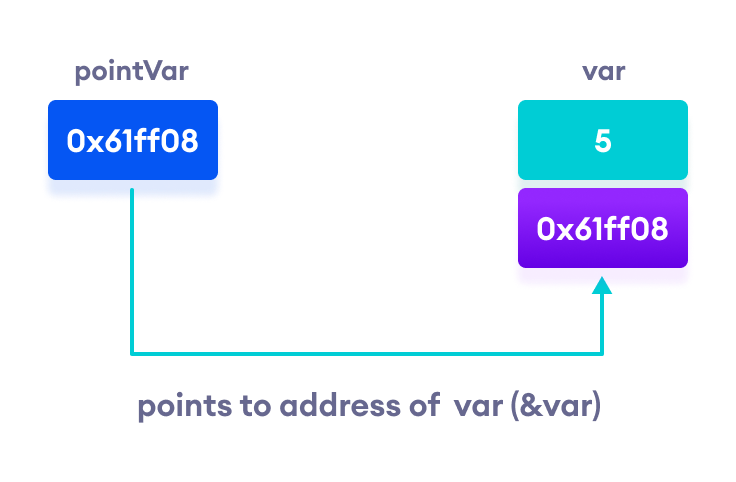
\includegraphics[width=4in]{images/cpp-pointer-working.png}
\caption{Working of C++ pointers}
\end{figure}

\doublelinewithspace{.0cm}

\hypertarget{changing-value}{%
\subsubsection{Changing Value Pointed by Pointers}\label{changing-value}}

If \texttt{pointVar} points to the address of \texttt{var}, we can
change the value of \texttt{var} by using \texttt{*pointVar}.

\textbf{For example,}
\begin{minted}[linenos]{c++}
int var = 5;
int* pointVar;

// assign address of var
pointVar = &var;

// change value at address pointVar
*pointVar = 1;

cout << var << endl; // Output: 1
\end{minted}

Here, \texttt{pointVar} and \texttt{\&var} have the same address, the
value of \texttt{var} will also be changed when \texttt{*pointVar} is
changed.

\doublelinewithspace{.0cm}

\hypertarget{example3}{%
\subsubsection{Example 3: Changing Value Pointed by
Pointers}\label{example3}}

\begin{minted}[linenos]{c++}
#include <iostream>
using namespace std;
int main() {
    int var = 5;
    int* pointVar;

    // store address of var
    pointVar = &var;

    // print var
    cout << "var = " << var << endl;

    // print *pointVar
    cout << "*pointVar = " << *pointVar << endl
         << endl;

    cout << "Changing value of var to 7:" << endl;

    // change value of var to 7
    var = 7;

    // print var
    cout << "var = " << var << endl;

    // print *pointVar
    cout << "*pointVar = " << *pointVar << endl
         << endl;

    cout << "Changing value of *pointVar to 16:" << endl;

    // change value of var to 16
    *pointVar = 16;

    // print var
    cout << "var = " << var << endl;

    // print *pointVar
    cout << "*pointVar = " << *pointVar << endl;
    return 0;
}
\end{minted}

\textbf{Output}
\begin{minted}[bgcolor=bg]{text}
var = 5
*pointVar = 5

Changing value of var to 7:
var = 7
*pointVar = 7

Changing value of *pointVar to 16:
var = 16
*pointVar = 16
\end{minted}

\doublelinewithspace{.0cm}

\hypertarget{common-mistakes}{%
\subsection{Common mistakes when working with pointers}\label{common-mistakes}}

Suppose, we want a pointer \texttt{varPoint} to point to the address of \texttt{var}. Then,

\begin{minted}[linenos]{c++}
int var, *varPoint;

// Wrong! 
// varPoint is an address but var is not
varPoint = var;

// Wrong!
// &var is an address
// *varPoint is the value stored in &var
*varPoint = &var;

// Correct! 
// varPoint is an address and so is &var
varPoint = &var;

 // Correct!
// both *varPoint and var are values
*varPoint = var;
\end{minted}

% \doublelinewithspace{.0cm}

% \textbf{Recommended Readings}:

% \begin{itemize}
% \tightlist
% \item
%   \href{/cpp-programming/pointer-void}{How to use generic data type
%   pointers using a void pointer?}
% \item
%   \href{/cpp-programming/pointers-arrays}{How to represent an array
%   using a pointer?}
% \item
%   \href{/cpp-programming/pointers-function}{How to use pointers with
%   functions?}
% \item
%   \href{/cpp-programming/structure-pointer}{How to use pointers with
%   structures?}
% \end{itemize}

% \href{/cpp-programming/operator-overloading}{}


\newpage
\mysection{Trees}

A graph is an ordered pair \textbf{\emph{G = (V, E)}} comprising a set \textbf{\emph{V}} of vertices, (aka: nodes or points) together with a set \textbf{\emph{E}} of edges, (aka: arcs or lines).\\

A tree is an \gls{undgraph} in which any two vertices are connected by exactly one path. In other words, any \gls{acyclic} connected graph is a tree.\\

Below is a directory tree. This is a tree that represents a portion of a file system on pretty much any operating system. It's a generic representation of a folder hierarchy, displaying subfolders, and files in folders. Notice that there is no restriction on the number of children. Nodes have from 1-4 children, and could have many more depending on how many items a folder were to contain. All trees represent relationships between items, this tree happens to represent folders and files. In academia we tend to lean toward very defined tree's (Binary Search Tree, \gls{btree}\supcite{Btree}, \gls{rtree}\supcite{Rtree}, \gls{marytree}\supcite{marytree}, \gls{trietree}\supcite{Trie}, and many more.) but these tree are nothing without the algorithms that define their properties and behaviors. This section is just to label components of generic trees. We will get into specifically defined trees later. 

\mysubsection{Tree Vocab}

\begin{center}
	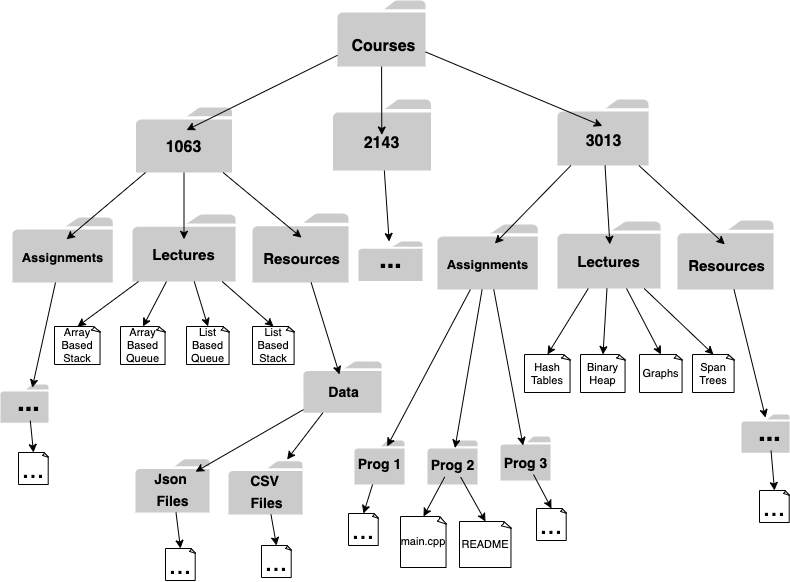
\includegraphics[scale=.45]{images/directory_structure_tree.png}
\end{center}

\begin{center}
	\begin{tabular}{p{0.1\textwidth} p{0.85\textwidth} }
		
		\textbf{Node}      &   
		A node is a fundamental part of a tree. It should contain information. Occasionally 
		all or part of the nodes data is called a  ``key.''  The key is a unique value we 
		use to perform comparisons when finding the proper location to place the node in the 
		tree. The node is not limited to storing only a key, in fact in the real world, it will
		store much more information in addition to the "key". Pretty much only in the classroom and
		books do we find trees that store  only "keys" (like an integer).\\
		\\
		\textbf{Edge}      &   
		An edge is another fundamental part of a tree. An edge connects two
		nodes to show that there is a relationship between them. Every node
		(except the root) is connected by exactly one incoming edge from
		another node. Each node may have several outgoing edges. For example
		in a binary tree, outgoing edges are limited to two edges, whereas in
		\gls{marytree} trees, the edges are limited to M where M is an integer $0 < m <= M$.\\
		\\
		\textbf{Root}      &   
		The root of the tree is the only node in the tree that has no
		incoming edges. It is the first node we look at in a binary tree. 
		\texttt{Courses} is the root in the file system tree.\\
		\\
		\textbf{Path}      &   
		A path is an ordered list of nodes that are connected by edges. For
		example, in the tree above: \texttt{Courses} $\rightarrow$ \texttt{3013}
		$\rightarrow$ \texttt{Assignments} $\rightarrow$ \texttt{Prog} 2 $\rightarrow$ \texttt{main.cpp} is a path.\\
		\\
		\textbf{Parent}    &   
		A node is the parent \texttt{P}, of all the nodes it connects to with outgoing
		edges. In the tree above the nodes \texttt{1063,2143,3013} are each parents to sub-folders \texttt{Assignments, Lectures, and Resources} (2143's children were collapsed for viewing).\\
		\\
		\textbf{Children}  &   
		The set of nodes \texttt{C} that have incoming edges from the same node \texttt{P},
		are said to be the children of that node. In the directory tree, \texttt{1063, 2143, 3013} are children of \texttt{Courses} (which also happens to be the root).\\
		\\
		\textbf{Sibling}   &   
		Nodes in the tree that are children of the same parent are said to
		be siblings. \texttt{1063, 2143, 3013} are siblings, as well as \texttt{Prog 1, Prog 2, Prog 3} are siblings (under \texttt{3013 $\rightarrow$ Assignments}).\\
		\\
		\textbf{Subtree}   &   
		A subtree is a set of nodes and edges comprised of a parent and all
		the descendants of that parent.\\
		\\
		\textbf{Leaf Node} &   
		A leaf node is a node that has no children. Look at the directory tree and notice all the "documents" are leaves. This not always the case (a folder could be empty and have no children). \\
		\\
		\textbf{Level}     &   
		The level of a node \texttt{N}  is the number of edges on the path from the
		root node to \texttt{N}. The level of Assignments (all of them) is level 2. The level of the README in Prog 2 is level 4.\\
		\\
		\textbf{Height}    &   
		The height of a tree is equal to the maximum level of any node in
		the tree. What is the height of this tree? It's not 4.\\
		
	\end{tabular}
\end{center}

% \begin{center}
% 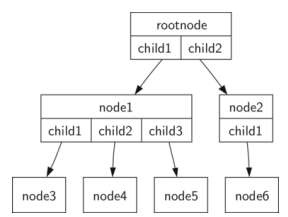
\includegraphics[scale=.5]{images/tree_edges_nodes.png}
% \end {center}


\newpage
\mysection{Binary Search Trees}


\begin{figure}[h]
 \centering
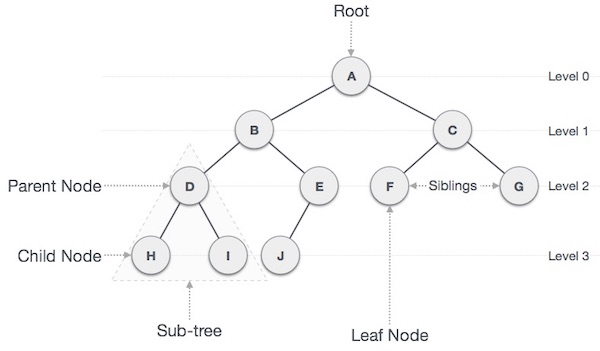
\includegraphics[scale=.6]{images/binary_tree.jpg}
\end{figure}

\mysubsection{Delete}

\mysubsubsection{Case 1: Zero Children}

Deleting a node with no children: remove the node from the tree.

\begin{figure}[h]
 \centering
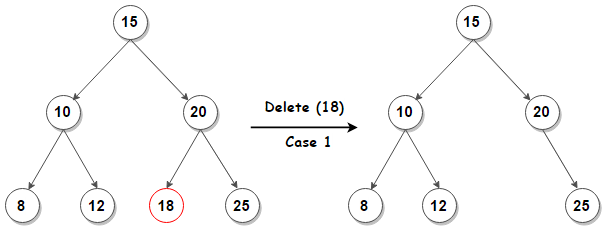
\includegraphics[scale=.6]{images/Deletion-in-BST-Case-1.png}
\end{figure}

\mysubsubsection{Case 2: Two Children}

Find the node to be deleted \textbf{N}. Do not delete \textbf{N}. Instead, choose either its  \lowercase{\gls{inordersucc}} node or its \gls{inorderpred} node, `R`. Copy the value of `R` to `N`, then recursively call delete on `R` until reaching one of the first two cases. If we choose the inorder successor of a node, as the right subtree is not NULL (our present case is a node with 2 children), then its inorder successor is a node with the least value in its right subtree, which will have at a maximum of 1 subtree, so deleting it would fall in one of the first 2 cases.


[inorder](https://www.techiedelight.com/inorder-tree-traversal-iterative-recursive/)
\newpage
\mysection{Traversals}


\mysubsection{Tree Traversals}

\mysubsubsection{Pre-Order}

\mysubsubsection{In-Order}

\mysubsubsection{Post-Order}

\mysubsubsection{Level-Order}

\mysubsection{Graph Traversals}

\mysubsubsection{Depth First Search}

\mysubsubsection{Breadth First Search}


\newpage
\mysection{Array Based Binary Tree}\label{abbst}\hypertarget{abbst}{}

When storing values in an array as if it were a \gls{bintree}, you use the current location: \textbf{i} and multiply it by 2 for the location of the left child, or multiply by 2 and add 1 for the location of the right child. For this reason, we ignore the $0^{th}$ location in the array, since zero multiplied by anything is ... well ... zero. \\

The table below shows us the calculations for \textit{Left Child}, \textit{Right Child}, and \textit{Parent} in the left column. The right column gives a visual example in which we can see that index \textbf{7} would have \textbf{3} as its parent ($i/2$ or $7/3$) and the left and right children of index \textbf{5} are \textbf{10} and \textbf{11} respectively ($2*5$ and $2*5+1$).

\mysubsubsection{Formulas}

\begin{center}
\begin{tabular}{|M{0.30\textwidth}|M{0.60\textwidth}|}
\hline
\textbf{Formulas} & \textbf{Visualization}\\
\hline
\begin{itemize}
\tightlist
\item Left Child \hspace{4.5mm}= $2 * i$
\item Right Child  \hspace{2mm}= $2 * i + 1$
\item Parent \hspace{1cm}= $i / 2$
\end{itemize}&
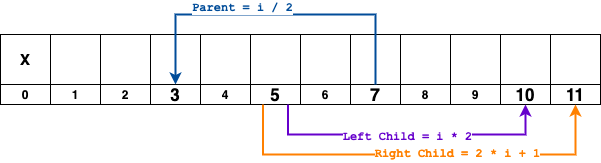
\includegraphics[scale=.4]{images/binary_tree_array_traversing.png} \\
\hline
\end{tabular}
\end{center}

\mysubsubsection{Example}
Below is an example inserting the values 13, 7 , 3, 17, 5, 11, 23 into an array based tree, along with it's binary tree equivalent. 

\begin{center}
\begin{tabular}{|M{0.10\textwidth}|M{0.50\textwidth} M{0.35\textwidth}|}
\hline
\textbf{Event} & \textbf{Array Based Tree} & \textbf{Binary Tree}\\
\hline
Insert 13 & 
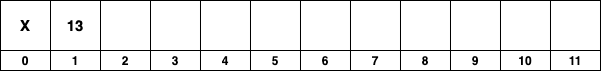
\includegraphics[scale=.4]{images/binary_tree_array_01.png} & 

\includegraphics[scale=.4]{images/binary_tree_example_01.png}\\
& \footnotesize{The root of the tree is empty. So location \textbf{1} gets the value.} &   \\
\hline
\end{tabular}
\end{center}
\begin{center}
\begin{tabular}{|M{0.10\textwidth}|M{0.50\textwidth} M{0.35\textwidth}|}
\hline
Insert 7 &
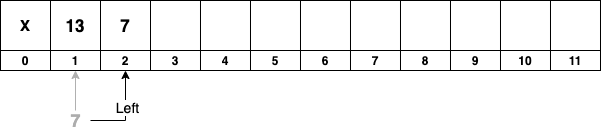
\includegraphics[scale=.4]{images/binary_tree_array_02.png} & 
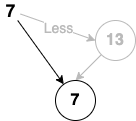
\includegraphics[scale=.4]{images/binary_tree_example_02.png}\\
& \footnotesize{7 is less than 13, go left. Its empty, store it there.} &   \\
\hline
\end{tabular}
\end{center}
\begin{center}
\begin{tabular}{|M{0.10\textwidth}|M{0.50\textwidth} M{0.35\textwidth}|}
\hline
Insert 17 &
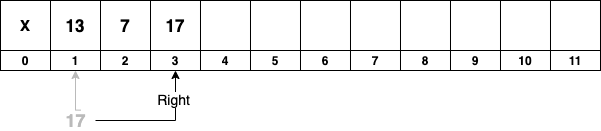
\includegraphics[scale=.4]{images/binary_tree_array_03a.png} & 
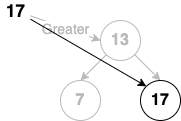
\includegraphics[scale=.4]{images/binary_tree_example_03.png}\\
& \footnotesize{17 is greater than 13, go right. Its empty, store it there.} &   \\
\hline
\end{tabular}
\end{center}
\begin{center}
\begin{tabular}{|M{0.10\textwidth}|M{0.50\textwidth} M{0.35\textwidth}|}
\hline
Insert 3 &
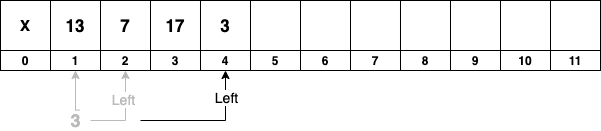
\includegraphics[scale=.4]{images/binary_tree_array_04a.png} & 
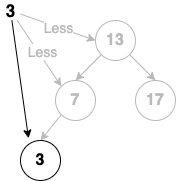
\includegraphics[scale=.4]{images/binary_tree_example_04.png}\\
& \footnotesize{3 is less than 13, go left. 3 is less than 7, go left. Its empty, store it there.} &   \\
\hline
\end{tabular}
\end{center}
\begin{center}
\begin{tabular}{|M{0.10\textwidth}|M{0.50\textwidth} M{0.35\textwidth}|}
\hline
Insert 5 &
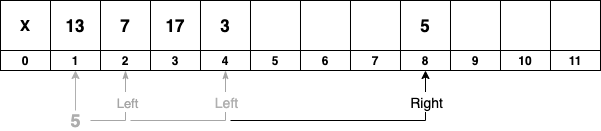
\includegraphics[scale=.4]{images/binary_tree_array_05.png} & 
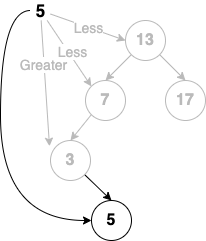
\includegraphics[scale=.4]{images/binary_tree_example_05.png}\\
& \footnotesize{5 is less than 13, go left. 5 is less than 7, go left. 5 is greater than 3, go right. Its empty, store it there.} &   \\
\hline
\end{tabular}
\end{center}
\begin{center}
\begin{tabular}{|M{0.10\textwidth}|M{0.50\textwidth} M{0.35\textwidth}|}
\hline
Insert 11 &
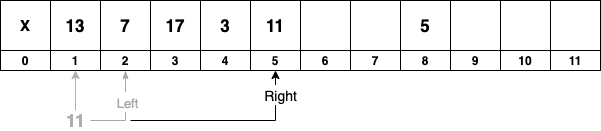
\includegraphics[scale=.4]{images/binary_tree_array_06.png} & 
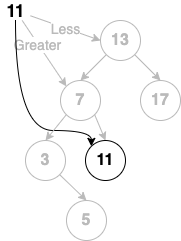
\includegraphics[scale=.4]{images/binary_tree_example_06.png}\\
& \footnotesize{11 is less than 13, go left. 11 is greater than 7, go right. Its empty, store it there.} &   \\
\hline
\end{tabular}
\end{center}
\begin{center}
\begin{tabular}{|M{0.10\textwidth}|M{0.50\textwidth} M{0.35\textwidth}|}
\hline
Insert 23 &
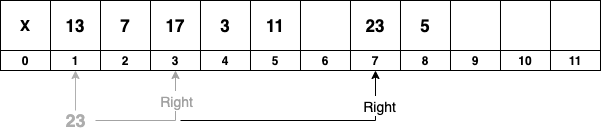
\includegraphics[scale=.4]{images/binary_tree_array_07.png} & 
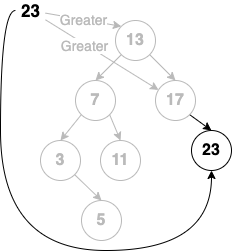
\includegraphics[scale=.4]{images/binary_tree_example_07.png}\\
& \footnotesize{23 is greater than 13, go right. 23 is greater than 17, go right. Its empty, store it there.} &   \\
\hline
\end{tabular}
\end{center}
\begin{center}
\begin{tabular}{|M{0.10\textwidth}|M{0.50\textwidth} M{0.35\textwidth}|}
\hline
Done &
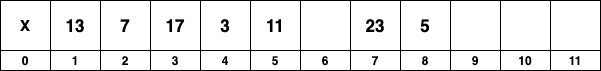
\includegraphics[scale=.4]{images/binary_tree_array_08.png} & 

\includegraphics[scale=.4]{images/binary_tree_example_08.png}\\
\hline
\end{tabular}
\end{center}

You can see the resulting array and tree above. Notice the empty slot at index 6. This is the type of thing you want to avoid with array based structures. One empty slot is not a big deal you say? Probably not. However, this is a small forced example. Why don't you continue this example on paper and insert the values 2 then 1. How big did you need to resize your array?\\

\newpage
\mysection{Heap Data Structure}

When you hear the term \textit{heap} your brain can go one of two ways: \gls{heapmemory} or \gls{heapds}. Early on in your CS career, you lean toward the memory version of a heap, since that is fresh on your brain. You just got through allocating dynamic memory with the "new" operator. Where does dynamic memory get stored? Well, the heap! However, this section is about a \gls{heapmemory} that allows for easy implementation of an efficient \gls{prioqueue}\supcite{Heapdata,Priority36}. So, are you wondering why we have a type of memory called "the heap" and a data structure call "a heap"? You aren't the only one. Donald Knuth said that back in 1975, several authors began to call the pool of available memory (not allocated to your process) a "heap"\supcite{knuth1997art}, but he never really clarified who or why. There are other "guesses" but it's not really clear. My opinion is that since "heap" has multiple meanings, it might just fit both scenarios.\\

\textbf{Heap Defintion:}
\begin{itemize}
	\tightlist
	\item n.	A group of things placed or thrown, one on top of the other.
	\item n.	A great deal; a lot.
\end{itemize}

A heap data structure is a group of items, placed one on top of another (with a special order to them), and heap memory could also refer to how the memory is allocated, OR to the excess memory not assigned to any process. Who knows?!? It's a conundrum.\\

This section will discuss the data structure variety that implements a priority queue. More specifically, we will describe an array based implementation of a binary heap. Because of how heap operations work, using an array to store values works. Even though it is possible to store a binary tree in an array, it doesn't mean that we should do it unless certain properties are maintained. If these properties are not maintained, its a sketchy situation at best. Meaning, lots of wasted space and empty slots. See section \hyperlink{abbst}{Array Based Binary Search Trees} for information on how to store a binary search tree in an array. 

\mysubsection{Array Based Binary Heap}

Knowing how to store values in an array as a binary search tree requires the programmer to implement certain algorithms. Likewise, to turn that array based binary tree into a binary heap, we must alter the algorithm (or operations) on how we interact with the data structure. It's the specific algorithms that we apply to generic containers (like an array) that makes them what they are. In the next section, we will take our simple binary search tree algorithm to another level when we add the functionality to implement a binary heap.\\

\mysubsubsection{Background}

A binary heap is a heap data structure that takes the form of a binary tree. The binary heap was introduced by J. W. J. Williams in 1964, as a data structure for  \gls{heapsort}\supcite{Binaryhe5}. It turns out, it could be used for more than sorting values. In fact heaps are a very good way of implementing \textbf{priority queues}'s. All we have to do with our binary tree to make it a heap is make sure that it fulfills the following properties:

\begin{enumerate}
	\tightlist
	\item It stays a \gls{complete} binary tree. 
	\item Each value stored in the tree is either less than or equal (Min Heap) or greater than or equal (Max Heap) to its parent. 
	\item If a child does not meet the previous property, it will be swapped with its parent.
\end{enumerate}

A heap data structure uses multiple methods to maintain its heap structure:

\begin{itemize}
	\tightlist
	\item Insert
	\item Remove 
	\item Heapify
	\item BubbleUp
	\item BubbleDown
\end{itemize}

\mysubsubsection{Overview}

In order to make our heap work efficiently, we will take advantage of the logarithmic nature of the binary tree to represent our heap. In order to guarantee logarithmic performance, we must keep our tree balanced\footnote{Go see the binary tree section for info about logarithmic performance.}. A tree is balanced if the difference of the left and right subtrees differ by no more than 1. We determine if the entire tree is balanced by looking at the height difference from the root's left and right subtrees.\\

We already mentioned we want our heap implementation to be a \gls{complete} binary tree. This means each level has all of its nodes. The exception to this is the bottom level of the tree, which we fill in from left to right. The Figure below shows an example of a complete binary tree with its array implementation.


\begin{figure}[h!]
	\centering
	\begin{subfigure}[b]{0.45\textwidth}
		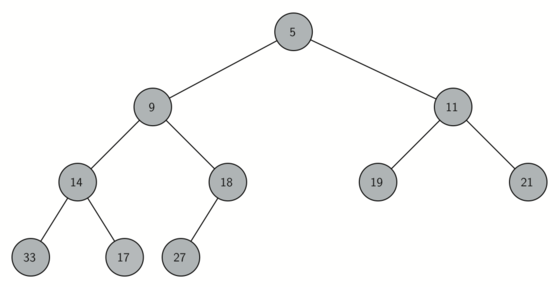
\includegraphics[width=\textwidth]{images/compTree_3013_2020.png}
		\caption{A Complete Binary Tree}
		\label{fig:compbintree}
	\end{subfigure}\\
	\vspace{.5cm}
	\begin{subfigure}[b]{0.45\textwidth}
		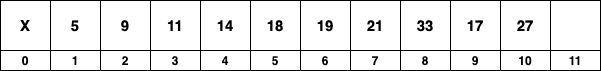
\includegraphics[width=\textwidth]{images/heap_array.png}
		\caption{Array Representation}
		\label{fig:arraytreerep}
	\end{subfigure}
	~ %add desired spacing between images, e. g. ~, \quad, \qquad, \hfill etc. 
	%(or a blank line to force the subfigure onto a new line)
	\caption{A Complete Tree and its Array Representation}\label{fig:arraybintreerep}
\end{figure}


How do we ensure that our heap implementation remains a complete tree? By using the array implementation we discussed above, and inserting new items into the tree by placing them into the next open element in the array. Look at the figure above. By inserting another value at array location 11, we give node 18 a right child, or node 27 a right sibling. Our tree stays "complete". If we were to expand our array and keep inserting into the next available slot, we would continue to fill the tree in from left to right at the bottom, until we started a new row. We never get "holes" in our array, and our tree stays complete and balanced. \\


\mysubsubsection{Heap Operations}

Even though we take advantage of an array based binary tree implementation, it doesn't mean we will insert items the same. In the array based binary tree we would compare our new value to the root of the tree, then find the location to store that value by comparing to the root, and then propagate \textbf{down} the tree moving left and right as needed (see figure \ref{fig:insbintree}).\\

% \begin{center}
% 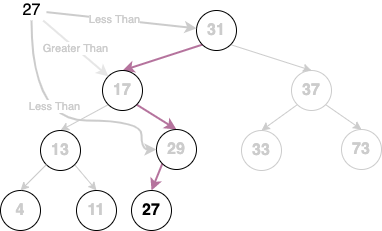
\includegraphics[scale=.45]{images/binary_tree_insert.png} 
% \end{center}

\begin{figure}[h!]
	\centering
	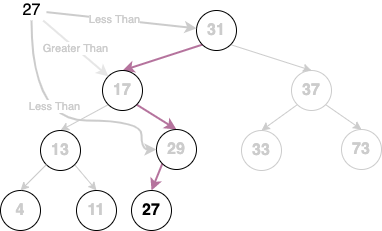
\includegraphics[width=.45\textwidth]{images/binary_tree_insert.png}
	\caption{Inserting into Binary Search Tree}
	\label{fig:insbintree}
\end{figure}

Because the heap property doesn't care about a total ordering of the tree, it only cares about the relationship between parent and child, we can insert values a little differently.\\

\mysubsubsubsection{Insert}

The easiest, and most efficient, way to add an item to a heap is to simply append the item to the next available slot in the array. The good news about this is that it will ALWAYS result in a complete tree. The bad news about appending is that we will very likely violate the heap structure property and have to re-arrange values based on whether it is a min-heap or a max-heap.\\


% \begin{SCfigure}
%     \centering
%     \begin{subfigure}[b]{0.45\textwidth}
%         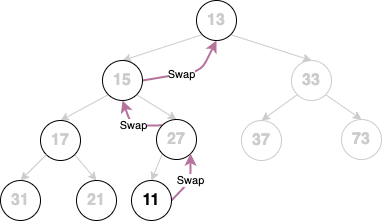
\includegraphics[width=\textwidth]{images/binary_heap_insert.png}
%         \caption{Bubbling Up}
%         \label{fig:heapinsert}
%     \end{subfigure}
%     \begin{subfigure}[b]{0.45\textwidth}
%         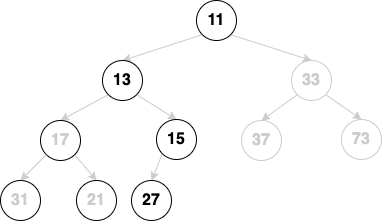
\includegraphics[width=\textwidth]{images/binary_heap_insert_2.png}
%         \caption{After Swaps}
%         \label{fig:heapresult}
%     \end{subfigure}
%     \caption{Inserting value into a heap}\label{fig:heapstuff}
% \end{SCfigure}

\begin{figure}[h!]
	\centering
	\begin{subfigure}[b]{0.45\textwidth}
		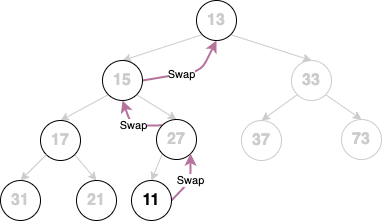
\includegraphics[width=\textwidth]{images/binary_heap_insert.png}
		\caption{Bubbling Up}
		\label{fig:heapinsert}
	\end{subfigure}
	\begin{subfigure}[b]{0.45\textwidth}
		\includegraphics[width=\textwidth]{images/binary_heap_insert_2.png}
		\caption{After Swaps}
		\label{fig:heapresult}
	\end{subfigure}
	\caption{Inserting value into a heap}\label{fig:heapstuff1}
\end{figure}

% \begin{minipage}{0.45\textwidth}
% \begin{figure}
%     \includegraphics[scale=.33]{images/binary_heap_insert.png}
%     \caption{ Heap Insert Bubble Up}
%     \label{fig:heapex1}
% \end{figure}
% \end{minipage}%
% \hfill%
% \begin{minipage}{0.45\textwidth}
%     \begin{figure}
%     \includegraphics[scale=.33]{images/binary_heap_insert_2.png}
%     \caption{Heap Bubble Up Result}
%     \label{fig:heapex2} 
%     \end{figure}
% \end{minipage}\\

% \begin{center}
% \begin{tabular}{|M{0.40\textwidth}|M{0.40\textwidth}|}
% \hline
% Heap Insert  & Heap Result  \\
% \hline
%   \begin{minipage}[t]{0.40\textwidth}
%     % \vspace{-2ex}

%   \end{minipage}
%  &
%   \begin{minipage}[t]{0.40\textwidth}
%     % \vspace{-2ex}

%   \end{minipage}\\
% \hline
% 11 gets placed at next available location in complete tree, and swaps its way up.&
% Resulting heap after all swaps made. \\
% \hline
% \end{tabular}
% \end{center}


Fixing any violations of the heap structure property can be done by comparing the newly added item with its parent. If the newly added item is less than its parent (assuming a min heap), then we can swap the item with its parent. Since the tree is always a complete tree and therefore balanced, we can assume worse case that an insert item will have to swap \texttt{O(lg n)} times. \\

In \textbf{figure \ref{fig:heapstuff1}} we see an example showing the series of swaps needed to percolate the newly added item up to its proper position in the tree. In table \ref{tab:exinsertheap} we can see the steps (using different values) broken down better.

\begin{center}
	\begin{table}
		\begin{tabular}{|p{0.20\textwidth}|M{0.4\textwidth}|M{0.30\textwidth}|}
			\hline
			  & Array & Binary Tree \\
			\hline
			Append to last slot. &
			\includegraphics[width=0.4\textwidth]{images/3013_heap_insert_1_2020.png}
			&
			\includegraphics[width=0.25\textwidth]{images/3013_heap_percup_1.png}\\
			\hline
			Swap with smaller parent. &
			\includegraphics[width=0.4\textwidth]{images/3013_heap_insert_2_2020.png}
			&
			\includegraphics[width=0.25\textwidth]{images/3013_heap_percup_2.png}\\
			\hline
			Swap with smaller parent (again). &
			\includegraphics[width=0.4\textwidth]{images/3013_heap_insert_3_2020.png}
			&
			\includegraphics[width=0.25\textwidth]{images/3013_heap_percup_3.png}\\
			\hline
		\end{tabular}
		\caption{Example insert showing comparisons while bubbling up.}
		\label{tab:exinsertheap}
	\end{table}
\end{center}

Notice that when we percolate an item up, we are restoring the heap property between the newly added item and the parent. We are also preserving the heap property for any siblings. Of course, if the newly added item is very small, we may still need to swap it up another level. In fact, we may need to keep swapping until we get to the top of the tree. \textbf{Figure \ref{fig:heapstuff1}} shows the \texttt{Bubble UP} or (percUp, siftUp, etc.) method, which swaps a new item as far up in the tree as it needs to go to maintain the heap property. Again, we use \textbf{\emph{i / 2}} to find the parent and swap the values if the child is smaller than the parent\footnote{Remember, this is a \textbf{minheap}, for \textbf{maxheap} we swap if child is larger.}.\\

\mysubsubsubsection{RemoveMin}

Since the heap property requires that the root of the tree be the smallest item in the tree, finding the minimum item is easy. The involved part of \texttt{RemoveMin} is restoring full compliance with the heap structure and heap order properties after the root has been removed. Restoring compliance can be solved in two simple steps: 1) A swap, and 2) a Bubble Down. More specifically:



\begin{enumerate}
	\def\labelenumi{\arabic{enumi}.}
	\tightlist
	\item
	      Swap the last item in the heap (from the back) to the top of the heap. 
	\item
	      Bubble this item down to its proper position since it will definitely ruin the heap order. 
\end{enumerate}

% \begin{center}
% \begin{tabular}{|p{0.20\textwidth}|M{0.4\textwidth}|M{0.30\textwidth}|}
% \hline
%  & Array & Binary Tree  \\
% \hline
% Append to last slot. &
% \includegraphics[width=0.4\textwidth]{images/3013_heap_insert_1_2020.png}
% &
% \includegraphics[width=0.25\textwidth]{images/3013_heap_percup_1.png}\\
% \hline

\begin{center}
	\begin{table}
		\begin{tabular}{|p{0.20\textwidth}|M{0.4\textwidth}|M{0.30\textwidth}|}
			\hline
			  & Array & Binary Tree \\
			\hline
			\scriptsize{Remove smallest value (5), swap with last item in array (27).}
			&
			\includegraphics[width=0.40\textwidth]{images/3013_heap_percdown_1_array.png}&
			\includegraphics[width=0.30\textwidth]{images/3013_heap_percdown_1.png}\\
			\hline
			\scriptsize{Then start to place the swapped value into it's proper location by comparing it to its children and restoring the heap property.}
			& 
			\includegraphics[width=0.40\textwidth]{images/3013_heap_percdown_2_array.png}&
			\includegraphics[width=0.30\textwidth]{images/3013_heap_percdown_2.png}\\
			\hline
		\end{tabular}
% 		\caption{Example insert showing comparisons while bubbling up.}
		\label{tab:removemin1}
	\end{table}
\end{center}

\begin{center}
	\begin{table}
		\begin{tabular}{|p{0.20\textwidth}|M{0.4\textwidth}|M{0.30\textwidth}|}
			\hline
			  & Array & Binary Tree \\
			\hline
			\scriptsize{Continue comparing and swapping as long as the heap property is violated (min-heap: parents must be smaller than their children).}
			& 
			\includegraphics[width=0.40\textwidth]{images/3013_heap_percdown_3_array.png}&
			\includegraphics[width=0.30\textwidth]{images/3013_heap_percdown_3.png}\\
			\hline
			\scriptsize{Stop swapping when no child is smaller, or there are no more children to compare to.}
			& 
			\includegraphics[width=0.40\textwidth]{images/3013_heap_percdown_4_array.png}&
			\includegraphics[width=0.30\textwidth]{images/3013_heap_percdown_4.png}\\
			\hline
		\end{tabular}
% 		\caption{Example insert showing comparisons while bubbling up.}
		\label{tab:removemin1}
	\end{table}
\end{center}


\mysubsubsubsection{Heapify}

To finish our discussion of binary heaps, we will look at a method to build an entire heap from an array of keys. If we insert items into the heap, one at a time we would get a performance of \textbf{\textit{O(n lg n)}}. Remember the height of a complete tree is \textbf{\textit{lg n}} (so each new item cannot bubble up further than \textit{lg n}). By inserting \textit{n} items, we get \textbf{\textit{O(n lg n)}} performance. However, if start with an unordered array of keys we can improve that time to 

Inserting n items gives us the first "n". And since we maintain a complete tree, it will be no taller than lg n, and so each can bubble up no further than lg n. 

The first method you might think of may be like the following. Given a list of keys, you could easily build a heap by inserting each key one at a time. Since you are starting with a list of one item, the list is sorted and you could use binary search to find the right position to insert the next key at a cost of approximately \textbf{\emph{O(lg n)}} operations. However, remember that inserting an item in the middle of the list may require \textbf{\emph{O(n)}} operations to shift the rest of the list over to make room for the new key. Therefore, to insert \textbf{\emph{n}} keys into the heap would require a total of \textbf{\emph{O(n lg n)}} operations. However, if we start with an entire list then we can build the whole heap in \textbf{\emph{O(n)}} operations.

\begin{center}
	\begin{table}
		\begin{tabular}{| p{0.25\textwidth}|M{0.30\textwidth}|M{0.35\textwidth}|}
			\hline
			  & Tree Representation & Array Representation \\
			\hline
			\scriptsize{Heapify: Starts with an array of unordered numbers.}
			&
			\includegraphics[scale=.30]{images/heapify_tree_01.png}
			&   
			\includegraphics[scale=.30]{images/heapify_01.png}\\
			\hline
		\end{tabular}
		% 		\caption{}
		% 		\label{heap:one}
	\end{table}
\end{center}

\begin{center}
	\begin{table}
		\begin{tabular}{| p{0.25\textwidth}|M{0.30\textwidth}|M{0.35\textwidth}|}
			\hline
			\scriptsize{We can ignore the bottom half of the array since all their children will be off the end of the array.}
			  &   
			\includegraphics[scale=.30]{images/heapify_tree_02.png}
			  &   
			\includegraphics[scale=.30]{images/heapify_02.png}\\
			\hline
		\end{tabular}
	\end{table}
\end{center}

\begin{center}
	\begin{table}
		\begin{tabular}{| p{0.25\textwidth}|M{0.30\textwidth}|M{0.35\textwidth}|}
			\hline
			\scriptsize{Find first location that has 1 or two children, and see if we need to swap (still assume min heap). Index 3 in this table our first candidate.}
			  &   
			\includegraphics[scale=.30]{images/heapify_tree_03.png}
			  &   
			\includegraphics[scale=.30]{images/heapify_03.png}\\
			\hline
		\end{tabular}
	\end{table}
\end{center}


\begin{center}
	\begin{table}
		\begin{tabular}{| p{0.25\textwidth}|M{0.30\textwidth}|M{0.35\textwidth}|}
			\hline
			\scriptsize{Make the swap with the smaller of the two children (11 < 19). 14 cannot bubble down any further so we stop.}
			  &   
			\includegraphics[scale=.30]{images/heapify_tree_04.png}
			  &   
			\includegraphics[scale=.30]{images/heapify_04.png}\\
			\hline
		\end{tabular}
	\end{table}
\end{center}


\begin{center}
	\begin{table}
		\begin{tabular}{| p{0.25\textwidth}|M{0.30\textwidth}|M{0.35\textwidth}|}
			\hline
			\scriptsize{We move up one index, and look at our children. Index 2 has children at locations 4 and 5.}
			  &   
			\includegraphics[scale=.30]{images/heapify_tree_05.png}
			  &   
			\includegraphics[scale=.30]{images/heapify_05.png}\\
			\hline
		\end{tabular}
	\end{table}
\end{center}


\begin{center}
	\begin{table}
		\begin{tabular}{| p{0.25\textwidth}|M{0.30\textwidth}|M{0.35\textwidth}|}
			\hline
			\scriptsize{We swap index 2 with the smallest of its children (5 < 9). 21 can bubble down no further so we stop.}
			  &   
			\includegraphics[scale=.30]{images/heapify_tree_06.png}
			  &   
			\includegraphics[scale=.30]{images/heapify_06.png}\\
			\hline
		\end{tabular}
	\end{table}
\end{center}


\begin{center}
	\begin{table}
		\begin{tabular}{| p{0.25\textwidth}|M{0.30\textwidth}|M{0.35\textwidth}|}
			\hline
			\scriptsize{We processed indexes 3 then 2 with minimal swapping. We still have index one to process.}
			  &   
			\includegraphics[scale=.30]{images/heapify_tree_07.png}
			  &   
			\includegraphics[scale=.30]{images/heapify_07.png}\\
			\hline
		\end{tabular}
	\end{table}
\end{center}


\begin{center}
	\begin{table}
		\begin{tabular}{| p{0.25\textwidth}|M{0.30\textwidth}|M{0.35\textwidth}|}
			\hline
			\scriptsize{We compare index 1 with its two children at indexes 2 and 3. }
			  &   
			\includegraphics[scale=.30]{images/heapify_tree_08.png}
			  &   
			\includegraphics[scale=.30]{images/heapify_08.png}\\
			\hline
		\end{tabular}
	\end{table}
\end{center}


\begin{center}
	\begin{table}
		\begin{tabular}{| p{0.25\textwidth}|M{0.30\textwidth}|M{0.35\textwidth}|}
			\hline
			\scriptsize{We swap index 1 with the smaller of its two children (5 < 11).}
			  &   
			\includegraphics[scale=.30]{images/heapify_tree_09.png}
			  &   
			\includegraphics[scale=.30]{images/heapify_09.png}\\
			\hline
		\end{tabular}
	\end{table}
\end{center}


\begin{center}
	\begin{table}
		\begin{tabular}{| p{0.25\textwidth}|M{0.30\textwidth}|M{0.35\textwidth}|}
			\hline
			\scriptsize{The value now at index 2 still has room to bubble down.}
			  &   
			\includegraphics[scale=.30]{images/heapify_tree_10.png}
			  &   
			\includegraphics[scale=.30]{images/heapify_10.png}\\
			\hline
		\end{tabular}
	\end{table}
\end{center}


\begin{center}
	\begin{table}
		\begin{tabular}{| p{0.25\textwidth}|M{0.30\textwidth}|M{0.35\textwidth}|}
			\hline
			\scriptsize{We again compare it to its children.}
			  &   
			\includegraphics[scale=.30]{images/heapify_tree_11.png}
			  &   
			\includegraphics[scale=.30]{images/heapify_11.png}\\
			\hline
		\end{tabular}
	\end{table}
\end{center}


\begin{center}
	\begin{table}
		\begin{tabular}{| p{0.25\textwidth}|M{0.30\textwidth}|M{0.35\textwidth}|}
			\hline
			\scriptsize{The value once again gets swapped with the smaller of its two children. So, this value bubbled down from the 1st index to the bottom of the tree (distance of lg n).} 
			  &   
			\includegraphics[scale=.30]{images/heapify_tree_12.png}
			  &   
			\includegraphics[scale=.30]{images/heapify_12.png}\\
			\hline
		\end{tabular}
	\end{table}
\end{center}


\begin{center}
	\begin{table}
		\begin{tabular}{| p{0.25\textwidth}|M{0.30\textwidth}|M{0.35\textwidth}|}
			\hline
            \scriptsize{We now have a valid min-heap.} 
			  &   
			\includegraphics[scale=.30]{images/heapify_tree_13.png}
			  &   
			\includegraphics[scale=.30]{images/heapify_13.png}\\
			\hline
		\end{tabular}
	\end{table}
\end{center}



% The figure above shows the swaps that the \texttt{Heapify} method makes as it moves the nodes in an initial tree of {[}9, 6, 5, 2, 3{]} into their proper positions. Although we start out in the middle of the tree and work our way back toward the root, the \texttt{percDown} method ensures that the largest child is always moved down the tree. Because the heap is a complete binary tree, any nodes past the halfway point will be leaves and therefore have no children. Notice that when \texttt{i=1}, we are percolating down from the root of the tree, so this may require multiple swaps. As you can see in the bottom most two trees in the figure above, first the 9 is moved out of the root position, but after 9 is moved down one level in the tree, \texttt{percDown} ensures that we check the next set of children farther down in the tree to ensure that it is pushed as low as it can go. In this case it results in a second swap with 3. Now that 9 has been moved to the lowest level of the tree, no further swapping can be done.

The assertion that we can build the heap in \textbf{\emph{O(n)}} may seem a bit mysterious at first, and were not proving anything. However, the key to understanding that you can build the heap in \textbf{\emph{O(n)}} is to remember that the \textbf{\emph{O(lg n)}} factor is derived from the height of the tree. For most of the work in \texttt{Heapify}, the tree is shorter than \textbf{\emph{lg n}}.

Using the fact that you can build a heap from a list in \textbf{\emph{O(n)}} time, you could easily construct a sorting algorithm that uses a heap and sorts a list in \textbf{\emph{O(n lg n)}} cost.
% \newpage
\mysection{Source Code}

% \inputminted
% [
% frame=lines,
% bgcolor=bg,
% framesep=2mm,
% baselinestretch=1.2,
% fontsize=\tiny,
% linenos
% ]
% {cpp}{sections/code_files/dijkstras.cpp}

\mysubsection{Graph Algorithms}

\begin{itemize}
    \item \href{https://gist.github.com/rugbyprof/2c213fc4cd22c7e398e46adac257fd3d}{Dijkstra's Algorithm}
    \item \href{https://gist.github.com/f4a854a92e05726189b859645e7b4609}{Breadth First Search}
    \item \href{https://gist.github.com/051202666be784cdb22e611e75d49ae2}{Connected Components}
    
\end{itemize}

\mysubsection{Hashing}

\begin{itemize}
    \item \href{https://gist.github.com/941937bb9a4104a5755e25d4fffc9cf5}{Chaining}
    \item \href{https://gist.github.com/dac58aea2c219efeee56d8d8d9487726}{Linear Probing}
    \item \href{https://gist.github.com/8de53804c1012f558344a5aede2d144d}{Quadratic Probing} 
    \item \href{https://gist.github.com/9cceec8c0653e3ec35ebf726325c5f7d}{Double Hashing}
\end{itemize}

\newpage
\hypertarget{uploading-to-uva-online-judge}{%
\mysection{Uploading to UVA Online Judge}\label{uploading-to-uva-online-judge}}

\begin{quote}
Adapted from Zachary Kingcades tutorial.
\end{quote}

\hypertarget{overview}{%
\mysubsection{Overview}\label{overview}}

There is a little different angle we must take when writing code to be
uploaded to https://onlinejudge.org/. Just like I have stressed in class
(oh remember the days when we had class \ldots) having a base knowledge
of the use of the command line can be beneficial. This tutorial will
discuss a couple of those skills and prepare you for uploading code to
UVA Online judge.

Keep in mind that solving these types of problems isn't just for
competition, its relevant for school and especially as a prep for
interviewing.

\hypertarget{registration-and-overview}{%
\mysubsubsection{Registration and Overview}\label{registration-and-overview}}

Onlinejudge has thousands of problems to browse and solve. You can look
at them without registering, but you will need to register to submit
solutions so go ahead and do that
\href{https://onlinejudge.org/index.php?option=com_comprofiler\&task=registers}{HERE}.

The major portion of Onlinejudge is its
\href{https://uhunt.onlinejudge.org/}{uHunt} section. This is where you
browse problems, submit your solutions, see statistics about each
problem, see latest submissions, and most importantly where you see the
status of your own submissions. You can click on the link I provided,
\textbf{or} look for this icon on the main page:

\begin{center}
\includegraphics[scale=.4]{images/uva_icon_sp_2020.png}\\
\end{center}

\hypertarget{selecting-a-problem}{%
\mysubsubsection{Selecting A Problem}\label{selecting-a-problem}}

You're registered, and ready to solve problems! How do you pick a
problem? There are many different ways and reasons to select a problem.

We are solving problems that require the understanding of specific data
structures as well as problem solving paradigms. Data structures
include: lists, arrays, stacks, queues, trees, graphs along with
variants or combos of each. Problem Solving Paradigms include: brute
force, divide and conquer, greedy, and dynamic programming.

We will use Competitive Programming 3 to help us choose problems that
will best be solved by choosing the proper data structure accompanied
with the correct problem solving paradigm.

\begin{quote}
\textbf{Note 1:} I hate stealing from any author, especially one who
created such a great resource. I'm sure he would understand our dilemma
this semester. I bought my own copy, and would encourage all of you to
\href{https://cpbook.net/\#CP3details}{purchase a copy}. Its a great
programming resource since it really concentrates on problem solving in
general, not just competitive programming.
\end{quote}

\begin{quote}
\textbf{Note 2:} The only reason I haven't used this from the beginning
is \ldots{} cheating :( You can find most of the solutions online. Even
though I have a defense for this, its just exhausting. More later
\ldots{}
\end{quote}

You don't only have to choose problems based on data structures and problem solving paradigms, believe it or not, people actually solve these for fun! I would recommend you solve as many of these as you have time for in addition to your course work. Lots of solutions will pad your resume` AND prepare you for interviews. So how do you choose problems to solve if its not for specific data structures? You can choose based on difficulty and how cool the name is. To do this, you have to \href{https://onlinejudge.org/index.php?option=com_onlinejudge\&Itemid=8}{browse} the problem sets. Below is the first menu of problems to choose from. We will concentrate on the two sets I placed a box around:

\begin{center}
\includegraphics[scale=.4]{images/brows_problems_sp_2020.png}
\end{center}

% \href{https://onlinejudge.org/index.php?option=com_onlinejudge\&Itemid=8}{\includegraphics[width=5.20833in,height=\textheight]{https://cs.msutexas.edu/~griffin/zcloud/zcloud-files/brows_problems_sp_2020.png}}

As you click folders, they drill down into other folders and finally lists of problems. If you drill down into any of the folders you will end up seeing something similar to below:

\begin{center}
\includegraphics[scale=.4]{images/problem_difficulty_sp_2020.png}
\end{center}

% \href{https://onlinejudge.org/index.php?option=com_onlinejudge\&Itemid=8\&category=6}{\includegraphics[width=5.20833in,height=\textheight]{https://cs.msutexas.edu/~griffin/zcloud/zcloud-files/problem_difficulty_sp_2020.png}}

We can see in a brief glance that lots of "red" = hard, and lots of "green" = easy (generally). The left column shows how many total submissions vs how many solved. In other words, lots of red means it takes many submissions before someone gets it correct. The right column is percentage of people that attempted the problem actually solved it. So, if you want an easy problem, find one that has a left column with 90+ solution percentage.

If you need to find a specific problem, they all have numbers (the ones we will use). So you can go \href{https://onlinejudge.org/index.php?option=com_onlinejudge\&Itemid=8}{browse} and find problems using the number to navigate folders, or you can go to \href{https://uhunt.onlinejudge.org/}{uHunt} and put the number in a search form (see \#1 on image).

\begin{center}
\includegraphics[scale=.4]{images/uhunt_browse_problems.png}
\end{center}

% \includegraphics[width=5.20833in,height=\textheight]{https://cs.msutexas.edu/~griffin/zcloud/zcloud-files/uhunt_browse_problems.png}

This will bring up a link to the problem description (see \#2 on image) which you can download and keep as a  reference as your solving. It also give you basic stats and current ``whats going on'' with the problem (see \#3 on image).

To stay organized I typically create a folder with the problem number as the folder name, and save everything from that associated problem in there. There will always be the pdf for the problem, multiple data sets to test your problem, and the actual source code. So, organizing with folders and problem numbers is recommended.

Aside from being organized and trying to decide what problems to solve, you really just need to break the ice and get a solution uploaded to uHunt. So lets start with a super easy one called \texttt{11172\ -\ Relational\ Operator}

\hypertarget{solving-a-problem}{%
\mysubsubsection{Solving A Problem}\label{solving-a-problem}}

You can refer to the previous section and go get the pdf of the problem we will solve. Its number is "11172". But for this tutorial, here are the contents:

\begin{center}\rule{0.5\linewidth}{0.5pt}\end{center}

\hypertarget{relational-operator}{%
\mysubsubsection{11172 - Relational Operator}\label{relational-operator}}

\begin{quote}
Time limit: 3.000 seconds
\end{quote}

Some operators checks about the relationship between two values and
these operators are called relational operators. Given two numerical
values your job is just to find out the relationship between them that
is (i) First one is greater than the second (ii) First one is less than
the second or (iii) First and second one is equal.

\hypertarget{input}{%
\paragraph{Input}\label{input}}

First line of the input file is an integer
\texttt{t\ (t\ \textless{}\ 15)} which denotes how many sets of inputs
are there. Each of the next \texttt{t} lines contain two integers
\texttt{a} and \texttt{b}
\texttt{(\textbar{}a\textbar{},\ \textbar{}b\textbar{}\ \textless{}\ 1000000001)}.

\hypertarget{output}{%
\paragraph{Output}\label{output}}

For each line of input produce one line of output. This line contains
any one of the relational operators \texttt{\textgreater{}},
\texttt{\textless{}} or \texttt{=}, which indicates the relation that is
appropriate for the given two numbers.

\hypertarget{sample-input}{%
\paragraph{Sample Input}\label{sample-input}}

\begin{verbatim}
3
10 20
20 10
10 10
\end{verbatim}

\hypertarget{sample-output}{%
\paragraph{Sample Output}\label{sample-output}}

\begin{verbatim}
<
>
=
\end{verbatim}

\begin{center}\rule{0.5\linewidth}{0.5pt}\end{center}

\hypertarget{coding-the-problem}{%
\mysubsubsection{Coding The Problem}\label{coding-the-problem}}

\hypertarget{start}{%
\paragraph{Start}\label{start}}

You should read over the problem and start to formulate a solution by
breaking it down into manageable components (more later). This problem
is easy. I will say, however, that initially none of the problems
\textbf{read} easy. They use mathematical notation to remove ambiguity
from the problem definition, and it is a bit confounding at first.
However it simply requires a little practice or a nice \textbf{slow}
approach to absorb its meaning.

\hypertarget{think}{%
\paragraph{Think}\label{think}}

For each problem we recommend that you THINK about it, re-read it, then
start your solution on paper. Also, when solving these problems, always
look at the limits as described in the problem
(e.g.~\texttt{t\ \textless{}\ 15} and
\texttt{(\textbar{}a\textbar{},\ \textbar{}b\textbar{}\ \textless{}\ 1000000001)}).
These could have an impact on the solution. For example, does
\texttt{1000000001} fit in an integer data type? Or should it be long?
Int works when uploaded for this solution, but on a tougher problem this
could bite you in the butt.

\hypertarget{code}{%
\paragraph{Code}\label{code}}

After you come up with a proposed solution, start to code it. Normal
coding conventions that we stress in class are a little out the window.
\textbf{Not all}, but some. Rules like self documenting variable names,
comments for each variable, organized procedural solution (lots of
functions) are all relaxed for these solutions.

\hypertarget{nuances}{%
\paragraph{Nuances}\label{nuances}}

Also, we want all the little speedups we can manage. \textbf{Example 1)}
in larger solutions where a function seems appropriate, you may want to
keep your code in main (inline), a function call is ever so slightly
slower than inline code. \textbf{Example 2)} Another miniscule speedup
is something as simple as re-defining \texttt{endl} to
\texttt{\textbackslash{}n}. The first one is interpreted as a newline
\textbf{AND} a flush of the output buffer. If one of the problems you
are solving has you writing to standard out thousands and thousands of
times, the extra flush may slow you down. Both of these are tiny little
speedups, but put a lot of those tiny speedups together, and it could
make a difference. Difference in what you ask? The first line after the
title in our problem statement states:
\texttt{Time\ limit:\ 3.000\ seconds}. That's the problem. Each solution
has a time limit to complete.

\hypertarget{stdin}{%
\paragraph{Stdin}\label{stdin}}

Lastly \textbf{cin} is NOT being used to prompt a user for input. It is
being used to read from an input file! Jump below the code and input
file \ldots{}

\begin{minted}[]{c++}
#include <iostream>

#define endl "\n"

using namespace std;

int  main(){
    int c,l,r,i=0;
    cin>>c;
     while(i<c){
         cin>>l>>r;
         if(l<r){
             cout<<'<'<<endl;
         }else if(l>r){
             cout<<'>'<<endl;
         }else{
             cout<<'='<<endl;
         }
         i++;
     }
     return 0;
}
\end{minted}


\hypertarget{infile}{%
\paragraph{infile}\label{infile}}

\begin{verbatim}
3
10 20
20 10
10 10
\end{verbatim}

\textbf{cin} reads from
\href{https://en.wikipedia.org/wiki/Standard_streams}{stdin} which means
a default connected stream for whatever platform you are on. Typically
when you run a program, and you need input, you pause execution of the
program with a \texttt{cin} and then it waits for input from the
``keyboard''. And when you write using \texttt{cout} it writes to
\texttt{stdout} which is usually the terminal (or dos window). As a side
note there is also \texttt{stderr} which is where errors are directed to
(we don't deal with stderr, as its usually used with log files and
such).

We change \texttt{stdin} to be input from a file. Why? If you upload
your code to be auto run, how do you process a file? You could be given
a path and a file name, but its actually easier to redirect a file into
your program.

Given:

\begin{itemize}
\tightlist
\item
  code is in \texttt{main.cpp}
\item
  we compile and its executable is now \texttt{main.exe}
\item
  we have an input file called \texttt{infile}
\end{itemize}

We can read \texttt{infile} using \texttt{cin} by doing:

\begin{verbatim}
./main.exe < infile 
\end{verbatim}

The command above says to take \texttt{infile} and send it into
\texttt{main.exe} as if we opened it, except we can use \texttt{cin} to
read from it. Basically, we changed \texttt{stdin} to be a file, instead
of the keyboard.

If you refer back to the code snippet, and infile, - line 9 reads in the
3, telling us how many ``pairs'' of values we need to read. - line 11
then reads in two values for every iteration of the loop

\hypertarget{run-in-visual-studio}{%
\mysubsubsection{Run in Visual Studio :(}\label{run-in-visual-studio}}

You have to edit the projects properties. So whichever side your
solution explorer is:

\begin{itemize}
\tightlist
\item
  Right Click on the Project and select Properties.
\item
  Project -\textgreater{} Properties -\textgreater{} Debugging
  -\textgreater{} Command Arguments
\item
  Add the following to your Command Arguments:
  \texttt{\textless{}\ input.txt}
\item
  Or something like that
\end{itemize}

\hypertarget{run-in-terminal}{%
\mysubsubsection{Run in Terminal}\label{run-in-terminal}}

A better way is to use command line and a bash console like
\texttt{gitbash}.

\begin{itemize}
\tightlist
\item
  Change into your folder with your code and input file.
\item
  Compile:

  \begin{itemize}
  \tightlist
  \item
    \texttt{g++\ \textless{}filename\textgreater{}\ -o\ \textless{}executablename\textgreater{}}
  \item
    \texttt{g++\ main.cpp\ -o\ main}
  \end{itemize}
\item
  Run:

  \begin{itemize}
  \tightlist
  \item
    \texttt{./main\ \textless{}\ inputfile}
  \end{itemize}
\end{itemize}

If you use any of the c++11 or later code constructs you will need to
set the compiler standard when compiling:

\begin{itemize}
\tightlist
\item
  Compile:

  \begin{itemize}
  \tightlist
  \item
    \texttt{g++\ -std=c++17\ main.cpp\ -o\ main}
  \item
    or replace c++17 with c++11 if thats what you need
  \end{itemize}
\end{itemize}

\hypertarget{repl.it}{%
\mysubsubsection{Repl.it}\label{repl.it}}

Repl.it is kinda awesome. Yes I said it. They give us a pretty nice
virtual linux environment to run our programs in. Basically, they give
us a virtual machine / command line solution \ldots{} in the browser. I
have the example from above here:
https://repl.it/{@rugbyprof/stdinexample}. Even if you don't have an
account it will let you run and edit that code. I would recommend
creating an account. Here is a tutorial on creating and using repl.it:
https://cs.msutexas.edu/replit\_tutorial/

\hypertarget{start-1}{%
\paragraph{Start}\label{start-1}}

\begin{itemize}
\tightlist
\item
  Click run so that it ``compiles'' first time.
\item
  You will have to stop it (see next pic)
\end{itemize}


\begin{center}
\includegraphics[scale=.4]{images/replit_stdin_1.png}
\end{center}

\hypertarget{stop}{%
\paragraph{Stop}\label{stop}}

\begin{itemize}
\tightlist
\item
  It will not finish, since its waiting for input:)
\item
  \texttt{cin} is still defined to read keyboard input, so hit the stop
  button.
\item
  You should see \texttt{exited,\ terminated} in the terminal.
\end{itemize}

\begin{center}
\includegraphics[scale=.4]{images/replit_stdin_2.png}
\end{center}

\hypertarget{test-run}{%
\paragraph{Test Run}\label{test-run}}

\begin{itemize}
\tightlist
\item
  When we hit ``run'' the first time , Replit compiled our code and made
  an executable with the same name as our file (minus the extension).
\item
  Since Replit is a linux virtual machine, we can run our program from
  the provided command line!
\item
  So, you can type \texttt{./main\ \textless{}\ input} in the terminal
  and get a correct run (notice we have output in the green box).
\end{itemize}

\begin{center}
\includegraphics[scale=.4]{images/replit_stdin_3.png}
\end{center}

\hypertarget{compile}{%
\paragraph{Compile}\label{compile}}

\begin{itemize}
\tightlist
\item
  We don't want to have to hit ``run'' to get a new executable every
  time we make a change to our source code. And we don't have to.
\item
  Again, Replit gives us a linux terminal, so let us compile our own
  code using the terminal they so nicely gave us.
\item
  So as you are testing your code, you can use the \texttt{up\ arrow} to
  cycle through the necessary commands (after you have typed them at
  least once).

  \begin{itemize}
  \tightlist
  \item
    Make a change, then using the terminal:
  \item
    Compile: \texttt{g++\ main.cpp\ -o\ main}
  \item
    Run: \texttt{./main\ \textless{}\ input}
  \end{itemize}
\end{itemize}

\begin{center}
\includegraphics[scale=.4]{images/replit_stdin_5.png}
\end{center}

\hypertarget{testing-your-solution}{%
\mysubsubsection{Testing Your Solution}\label{testing-your-solution}}

You can now run your code using an input file as stdin. But how do we
know if the solution is correct? You know its correct if:

\begin{itemize}
\tightlist
\item
  You thought of every edge case possible.
\item
  You incorporated all nuances of the problem description into your
  solution.
\item
  Your output is formatted perfectly.
\item
  You are smarter than anyone you know.
\end{itemize}

The problem is, you really do not know if your solution is correct. You
can upload it to uHunt and roll the dice to see if your solution will be
accepted. Or, you can try to ensure your solution is correct by running
multiple test data sets.

If you go to the problems page where you got the pdf from, you will see
a lady bug at the top right above the problem statement. Click on it. It
will take you from
\href{https://onlinejudge.org/index.php?option=com_onlinejudge\&Itemid=8\&category=24\&page=show_problem\&problem=2113}{uHunt}
to \href{https://www.udebug.com/UVa/11172}{uDebug} where you have some
options for testing your solution more thoroughly using data sets
uploaded by other users. They go way beyond the example data given in
the problem, and will help you determine if you really did thing about
all the ``edge cases'' that might appear in the data.

\hypertarget{go-debug}{%
\paragraph{Go Debug}\label{go-debug}}


\begin{center}
\includegraphics[scale=.4]{images/replit_debug_sp_2020.png}
\end{center}

\hypertarget{getting-data}{%
\paragraph{Getting Data}\label{getting-data}}

\begin{itemize}
\tightlist
\item
  When you go to the debug site for your problem, you will see multiple
  data sets to choose from as I enclosed in a box.
\item
  Above the blue box, you will see a link to the most popular input
  data. But all of them should help you debug.
\item
  If your code can process all of the data sets, you should be good (but
  not always :) I have one solution that passed ALL data sets but fails
  online. )
\end{itemize}

\begin{center}
\includegraphics[scale=.4]{images/uhunt_debug_get_data.png}
\end{center}

\hypertarget{pick-a-set}{%
\paragraph{Pick a Set}\label{pick-a-set}}

\begin{enumerate}
\def\labelenumi{\arabic{enumi}.}
\tightlist
\item
  Pick a data set
\item
  Copy it to your clipboard
\end{enumerate}


\begin{center}
\includegraphics[scale=.4]{images/uhunt_debug_copy_data.png}
\end{center}

\hypertarget{use-new-data}{%
\paragraph{Use New Data}\label{use-new-data}}

\begin{enumerate}
\def\labelenumi{\arabic{enumi}.}
\tightlist
\item
  Create a new file
\item
  Paste new data in file
\item
  Run your code with new data file
\end{enumerate}

\begin{quote}
Your new output will be in the terminal, you need to copy it to bring
back to uDebug.
\end{quote}

\begin{center}
\includegraphics[scale=.3]{images/uhunt_rerun_newdata.png}
\end{center}

\hypertarget{check-new-output}{%
\paragraph{Check New Output}\label{check-new-output}}

\begin{enumerate}
\def\labelenumi{\arabic{enumi}.}
\tightlist
\item
  Click to get accepted output.
\item
  This window shows whats expected.
\item
  This is where you paste your output to be compared with accepted
  output.
\item
  Click to see if it matches!
\end{enumerate}

\begin{quote}
Note: uDebug gives better feedback than simply uploading your solution.
In fact lots of times solutions are rejected for an extra ``newline''.
This can be fixed here at uDebug.
\end{quote}


\begin{center}
\includegraphics[scale=.4]{images/uhunt_results_newdata.png}
\end{center}

\hypertarget{uploading-solution}{%
\mysubsubsection{Uploading Solution}\label{uploading-solution}}

\hypertarget{start-submission}{%
\paragraph{Start Submission}\label{start-submission}}

\begin{itemize}
\tightlist
\item
  Go back to the problem page and click on submit.
\end{itemize}

\begin{center}
\includegraphics[scale=.4]{images/uhunt_choose_submit.png}
\end{center}

\hypertarget{do-submission}{%
\paragraph{Do Submission}\label{do-submission}}

\begin{itemize}
\tightlist
\item
  On the next page:

  \begin{itemize}
  \tightlist
  \item
    Choose your version of c++
  \item
    Paste your code into the submission text field or Upload a file.
  \item
    Press ``submit''
  \end{itemize}
\end{itemize}


\begin{center}
\includegraphics[scale=.4]{images/uhunt_paste_code_submit.png}
\end{center}

\hypertarget{confirm-submission}{%
\paragraph{Confirm Submission}\label{confirm-submission}}

\begin{itemize}
\tightlist
\item
  You Get redirected back to the problem page with a confirmation.
\end{itemize}

\begin{center}
\includegraphics[scale=.4]{images/uhunt_confirm_submit.png}
\end{center}

\hypertarget{submission-results}{%
\paragraph{Submission Results}\label{submission-results}}

\begin{itemize}
\tightlist
\item
  You will get an email telling you what happened, but I like to view
  the stats on the website.
\item
  On the main onlinejudge site.
\item
  Click on last 50 submissions (under site statistics).
\item
  You should see your results (if you don't wait too long).
\end{itemize}

\begin{center}
\includegraphics[scale=.4]{images/uhunt_see_results.png}
\end{center}
\newpage
\mysection{ AVL Trees}

Copied From TutorialsPoint \href{https://www.tutorialspoint.com/data_structures_algorithms/avl_tree_algorithm.htm}{AvlTrees} \supcite{DataStru95:online}\\

What if the input to binary search tree comes in a sorted (ascending or descending) manner? It will then look like this:

\begin{center}
\includegraphics[scale=.60]{images/unbalanced_bst.jpg}
\end{center}

It is observed that BST's worst-case performance is closest to linear search algorithms, that is Ο(n). In real-time data, we cannot predict data pattern and their frequencies. So, a need arises to balance out the existing BST.\\

Named after their inventor \textbf{Adelson}, \textbf{Velski} \& \textbf{Landis}, \textbf{AVL trees} are height balancing binary search tree. AVL tree checks the height of the left and the right sub-trees and assures that the difference is not more than 1. This difference is called the \ccb{Balance Factor}.\\

Here we see that the first tree is balanced and the next two trees are not balanced −

\begin{center}
\includegraphics[scale=.60]{images/unbalanced_avl_trees.jpg}
\end{center}

In the second tree, the left subtree of \textbf{C} has height 2 and the right subtree has height 0, so the difference is 2. In the third tree, the right subtree of \textbf{A} has height 2 and the left is missing, so it is 0, and the difference is 2 again. AVL tree permits difference (balance factor) to be only 1.

\begin{verbatim}
BalanceFactor = height(left-sutree) − height(right-sutree)
\end{verbatim}

If the difference in the height of left and right sub-trees is more than \ccb{1}, the tree is balanced using some rotation techniques.

\newpage
\hypertarget{avl-rotations}{%
\mysubsection{AVL Rotations}\label{avl-rotations}}

To balance itself, an AVL tree may perform the following four kinds of rotations −

\begin{itemize}
\tightlist
\item
  Left rotation
\item
  Right rotation
\item
  Left-Right rotation
\item
  Right-Left rotation
\end{itemize}

The first two rotations are single rotations and the next two rotations are double rotations. To have an unbalanced tree, we at least need a tree of height 2. With this simple tree, let's understand them one by one.

\hypertarget{left-rotation}{%
\mysubsubsection{Left Rotation}\label{left-rotation}}

If a tree becomes unbalanced, when a node is inserted into the right subtree of the right subtree, then we perform a single left rotation −

\begin{center}
\includegraphics[scale=.60]{images/avl_left_rotation.jpg}
\end{center}

In our example, node \textbf{A} has become unbalanced as a node is inserted in the right subtree of A's right subtree. We perform the left rotation by making \textbf{A} the left-subtree of B.

\hypertarget{right-rotation}{%
\mysubsubsection{Right Rotation}\label{right-rotation}}

AVL tree may become unbalanced, if a node is inserted in the left subtree of the left subtree. The tree then needs a right rotation.

\begin{center}
\includegraphics[scale=.60]{images/avl_right_rotation.jpg}
\end{center}

As depicted, the unbalanced node becomes the right child of its left child by performing a right rotation.

\hypertarget{left-right-rotation}{%
\mysubsubsection{Left-Right Rotation}\label{left-right-rotation}}

Double rotations are slightly complex version of already explained versions of rotations. To understand them better, we should take note of each action performed while rotation. Let's first check how to perform Left-Right rotation. A left-right rotation is a combination of left rotation followed by right rotation.

\begin{longtable}{| M{.20\textwidth} | p{.80\textwidth} |} 
% \begin{table}[H]
\hline
\textbf{State} & \textbf{Action} \\
\hline
\includegraphics[scale=.40]{images/right_subtree_of_left_subtree.jpg} & A node has been inserted into the right subtree of the left subtree. This makes \textbf{C} an unbalanced node. These scenarios cause AVL tree to perform left-right rotation. \\ 
\hline
\includegraphics[scale=.40]{images/subtree_left_rotation.jpg} & We first perform the left rotation on the left subtree of \textbf{C}. This makes \textbf{A}, the left subtree of \textbf{B}. \\ 
\hline
\includegraphics[scale=.40]{images/left_unbalanced_tree.jpg} & Node \textbf{C} is still unbalanced, however now, it is because of the left-subtree of the left-subtree. \\ 
\hline
\includegraphics[scale=.40]{images/right_rotation.jpg} & We shall now right-rotate the tree, making \textbf{B} the new root node of this subtree. \textbf{C} now becomes the right subtree of its own left subtree. \\ 
\hline
\includegraphics[scale=.40]{images/balanced_avl_tree.jpg} & The tree is now balanced. \\ 
\hline
\end{longtable}

\hypertarget{right-left-rotation}{%
\mysubsubsection{Right-Left Rotation}\label{right-left-rotation}}

The second type of double rotation is Right-Left Rotation. It is a
combination of right rotation followed by left rotation.

\begin{longtable}{| M{.20\textwidth} | p{.80\textwidth} |} 
% \begin{table}[H]
\hline
\textbf{State} & \textbf{Action} \\
\hline
\includegraphics[scale=.40]{images/left_subtree_of_right_subtree.jpg} & A node has been inserted into the left subtree of the right subtree. This makes \textbf{A}, an unbalanced node with balance factor 2.\\
\hline
\includegraphics[scale=.40]{images/subtree_right_rotation.jpg} & First, we perform the right rotation along \textbf{C} node, making \textbf{C} the right subtree of its own left subtree \textbf{B}. Now, \textbf{B} becomes the right subtree of \textbf{A}. \\
\hline
\includegraphics[scale=.40]{images/right_unbalanced_tree.jpg} & Node \textbf{A} is still unbalanced because of the right subtree of its right subtree and requires a left rotation.\\
\hline
\includegraphics[scale=.40]{images/left_rotation.jpg} & A left rotation is performed by making \textbf{B} the new root node of the subtree. \textbf{A} becomes the left subtree of its right subtree \textbf{B}. \\
\hline
\includegraphics[scale=.50]{images/balanced_avl_tree.jpg} & The tree is now balanced.
\hline
\end{longtable}
\newglossaryentry{heapds}{
    name=heap data structure,
    description=A type of data structure that efficiently implements a priority queue using a binary structure in an array. It can also be used to sort numbers
}

\newglossaryentry{heapmemory}{
    name=heap memory,
    description=A type of memory that is typically associated with dynamically allocated data, and exists throughout the lifetime of your program
}

\newglossaryentry{prioqueue}{
    name=priority queue,
    description=A queue like data structure in which an element with high priority gets preference (removed or served) before an element with lower priority
}

\newglossaryentry{bintree}{
    name=binary tree,
    description=A binary tree is a tree data structure in which each node has at most two children, which are referred to as the left child and the right child
}

\newglossaryentry{heapsort}{
    name=heapsort,
    description=Sorting values using a binary heap by inserting the values into a heap and then removing the items 1 by 1 
}

\newglossaryentry{complete}{
    name=complete,
    description={In terms of a binary tree, All levels except possibly the last one (deepest) are fully filled, and, if the last level of the tree is not complete, the nodes of that level are filled from left to right}
}

\newglossaryentry{acyclic}{
    name=acyclic,
    description={In terms of a graph, acyclic means that there are no cycles in the graph}
}

\newglossaryentry{undgraph}{
    name=undirected graph,
    description={In a graph, G = (V, E), none of the edges have an "orientation" (no direction associated with the edge). This means
    that we can traverse an edge $A-B$ from $A \rightarrow B$ or from $B \rightarrow A$. Given a directed edge (one with orientation) and an edge $A \rightarrow B$, we can only traverse this edge in that direction, and \textbf{not} from $B \rightarrow A$}
}


\newglossaryentry{marytree}{
    name=m-ary tree,
    description={In graph theory, an m-ary tree (also known as k-ary or k-way tree) is a rooted tree in which each node has no more than m children. A binary tree is the special case where m = 2, and a ternary tree is another case with m = 3 that limits its children to three}
}

\newglossaryentry{trietree}{
    name=trie,
    description={In computer science, a trie, also called digital tree or prefix tree, is a kind of search tree—an ordered tree data structure used to store a dynamic set or associative array where the keys are usually strings. Unlike a binary search tree, no node in the tree stores the key associated with that node; instead, its position in the tree defines the key with which it is associated; i.e., the value of the key is distributed across the structure. All the descendants of a node have a common prefix of the string associated with that node, and the root is associated with the empty string. Keys tend to be associated with leaves, though some inner nodes may correspond to keys of interest. Hence, keys are not necessarily associated with every node}
}

\newglossaryentry{btree}{
    name=b-tree,
    description={In computer science, a B-tree is a self-balancing tree data structure that maintains sorted data and allows searches, sequential access, insertions, and deletions in logarithmic time. The B-tree generalizes the binary search tree, allowing for nodes with more than two children. Unlike other self-balancing binary search trees, the B-tree is well suited for storage systems that read and write relatively large blocks of data, such as disks. It is commonly used in databases and file systems}
}

\newglossaryentry{rtree}{
    name=r-tree,
    description={R-trees are tree data structures used for spatial access methods, i.e., for indexing multi-dimensional information such as geographical coordinates, rectangles or polygons. The R-tree was proposed by Antonin Guttman in 1984 and has found significant use in both theoretical and applied contexts. A common real-world usage for an R-tree might be to store spatial objects such as restaurant locations or the polygons that typical maps are made of: streets, buildings, outlines of lakes, coastlines, etc. and then find answers quickly to queries such as "Find all museums within 2 km of my current location", "retrieve all road segments within 2 km of my location" (to display them in a navigation system) or "find the nearest gas station" (although not taking roads into account). The R-tree can also accelerate nearest neighbor search for various distance metrics, including great-circle distance}
}

\newglossaryentry{tcomplex}{
    name=time complexity,
    description={In computer science, the time complexity is the computational complexity that describes the amount of computer time it takes to run an algorithm. Time complexity is commonly estimated by counting the number of elementary operations performed by the algorithm, supposing that each elementary operation takes a fixed amount of time to perform. Thus, the amount of time taken and the number of elementary operations performed by the algorithm are taken to differ by at most a constant factor}
}

\newglossaryentry{spacecomplex}{
name=space complexity,
description={The space complexity of an algorithm or a computer program is the amount of memory space required to solve an instance of the computational problem as a function of characteristics of the input. It is the memory required by an algorithm to execute a program and produce output}
}

\newglossaryentry{asymptotic}{
name=asymptotic notation,
description={ Big O notation is a mathematical notation that describes the limiting behavior of a function when the argument tends towards a particular value or infinity. Big O is a member of a family of notations invented by Paul Bachmann,[1] Edmund Landau,[2] and others, collectively called Bachmann–Landau notation or asymptotic notation}
}

\newglossaryentry{treetraversal}{
name=tree traversal,
description={Tree traversal (also known as tree search and walking the tree) is a form of graph traversal and refers to the process of visiting (checking and/or updating) each node in a tree data structure, exactly once. Such traversals are classified by the order in which the nodes are visited. The following algorithms are described for a binary tree, but they may be generalized to other trees as well}
}


\newglossaryentry{inordersucc}{
name=in order successor,
description={In a binary search tree, the in order successor of some node \textit{N}, can also be defined as the node with the smallest key greater than the key of \textit{N}. Or it is smallest value in the right sub-tree of node \textit{N}}
}

\newglossaryentry{inorderpred}{
name=in order predecessor,
description={In a binary search tree, the in order predecessor of some node \textit{N}, can also be defined as the node with the largest key smaller than the key of \textit{N}. Or it is largest value in the left sub-tree of node \textit{N}}
}




\newglossaryentry{term}{
name=What Shows,
description={}
}


% Bibliography
% \newpage
% \nocite{*}
\newpage
% \printbibliography[heading=bibintoc]
\bibliography{main}
\glsresetall

%Print the glossary
\printglossaries

\end{document}

